\section{Mathematical Preliminaries}
\label{appendix:mathprelim}

This appendix collects the mathematical results the survey rests on but does not develop in the main text. It assumes only probability, calculus, and linear algebra at the level of a first graduate sequence. From there it builds the handful of tools that recur across the chapters. The contraction-mapping principle drives every dynamic-programming convergence proof. Stochastic approximation underlies every claim that a sampled iterate converges to its target. Convex analysis and duality support policy optimization and constrained control. A few probability and matrix facts carry the estimation and Markov-chain arguments. Each result is stated, proved, and illustrated by a small simulation. The chapters point here in a footnote wherever they use one of these results, and each result points back to the chapters that use it. The material runs in four parts. They cover linear algebra and matrix analysis, probability, calculus and convex analysis, and the fixed-point and stochastic-approximation results that bridge to dynamic programming.

\subsection{Linear Algebra and Matrix Analysis}
\label{prelim:linalg}

The value of a policy is a vector, the Bellman update is a matrix acting on it, and the long-run behavior of a Markov chain is an eigenvector. Four facts about matrices carry these arguments. The first says when repeated multiplication drives a vector to zero. The second writes the value function as a geometric series. The third pins down the long-run state distribution. The fourth is the projection geometry behind linear function approximation.

\subsubsection{Spectral Radius and Decay of Matrix Powers}

\begin{theorem}[Spectral radius governs decay, \citet{hornjohnson2013}]
\label{thm:prelim_spectral}
Let $A$ be a square matrix with spectral radius $\rho(A) = \max_i |\lambda_i|$, the largest modulus among its eigenvalues.\footnote{An \emph{eigenvalue} $\lambda$ of $A$ is a number for which $Av = \lambda v$ has a nonzero solution $v$, the \emph{eigenvector}. Applying $A$ to $v$ just rescales it by $\lambda$. The \emph{spectral radius} is the largest such $|\lambda|$.} Then the matrix powers vanish, $A^k \to 0$ as $k \to \infty$, if and only if $\rho(A) < 1$. In that case $\|A^k\|^{1/k} \to \rho(A)$.
\end{theorem}

\begin{proof}
The plan is to read both directions off the eigenvalues, using an eigenvector for the ``only if'' part and the Jordan form for the ``if'' part. Suppose first $\rho(A) \geq 1$. Pick an eigenvalue with $|\lambda| \geq 1$ and a unit eigenvector $v$. Then
\begin{align*}
\|A^k v\| = \|\lambda^k v\| = |\lambda|^k \geq 1 && \text{(eigenvector, $|\lambda| \geq 1$),}
\end{align*}
so $A^k$ does not converge to $0$. Now suppose $\rho(A) < 1$. Write $A = S J S^{-1}$ in Jordan form.\footnote{Every square matrix is similar to a block-diagonal \emph{Jordan form} $J$, whose blocks are $\lambda I + N$ with $N$ nilpotent, meaning $N^m = 0$ for some $m$. Powers of $A$ and of $J$ differ only by the fixed change of basis $S$.} It is enough to show each block $J_i = \lambda I + N$ satisfies $J_i^k \to 0$. Expanding the power,
\begin{align*}
J_i^k = (\lambda I + N)^k
  &= \sum_{j=0}^{m-1} \binom{k}{j} \lambda^{k-j} N^j && \text{(binomial, $N^m = 0$)} \\
  \|J_i^k\| &\leq \sum_{j=0}^{m-1} \binom{k}{j} |\lambda|^{k-j} \|N\|^j && \text{(triangle inequality).}
\end{align*}
Each term is a polynomial in $k$ times $|\lambda|^k$. Since $|\lambda| < 1$, the exponential $|\lambda|^k$ beats every polynomial, so each term tends to $0$. Thus $J_i^k \to 0$, hence $A^k = S J^k S^{-1} \to 0$. The rate claim $\|A^k\|^{1/k} \to \rho(A)$ follows because the dominant term above grows like $k^{m-1} \rho(A)^k$, whose $k$-th root tends to $\rho(A)$.
\end{proof}

The distinction between $\rho(A)$ and the norm $\|A\|$ matters in practice.\footnote{The spectral radius sets the target-network and composed-operator stability conditions of Section~\ref{sec:planning_learning} and the low-rank and manipulation-cost arguments of Section~\ref{section:bandits}.} A matrix can have $\|A\| > 1$, so its powers grow at first, yet still decay because $\rho(A) < 1$. Figure~\ref{fig:prelim_spectral} shows this transient for a non-normal matrix. The powers rise to a peak, then fall, and the per-step decay ratio settles at $\rho(A)$ (Table~\ref{tab:prelim_spectral_radius}).

\begin{figure}[t]
\centering
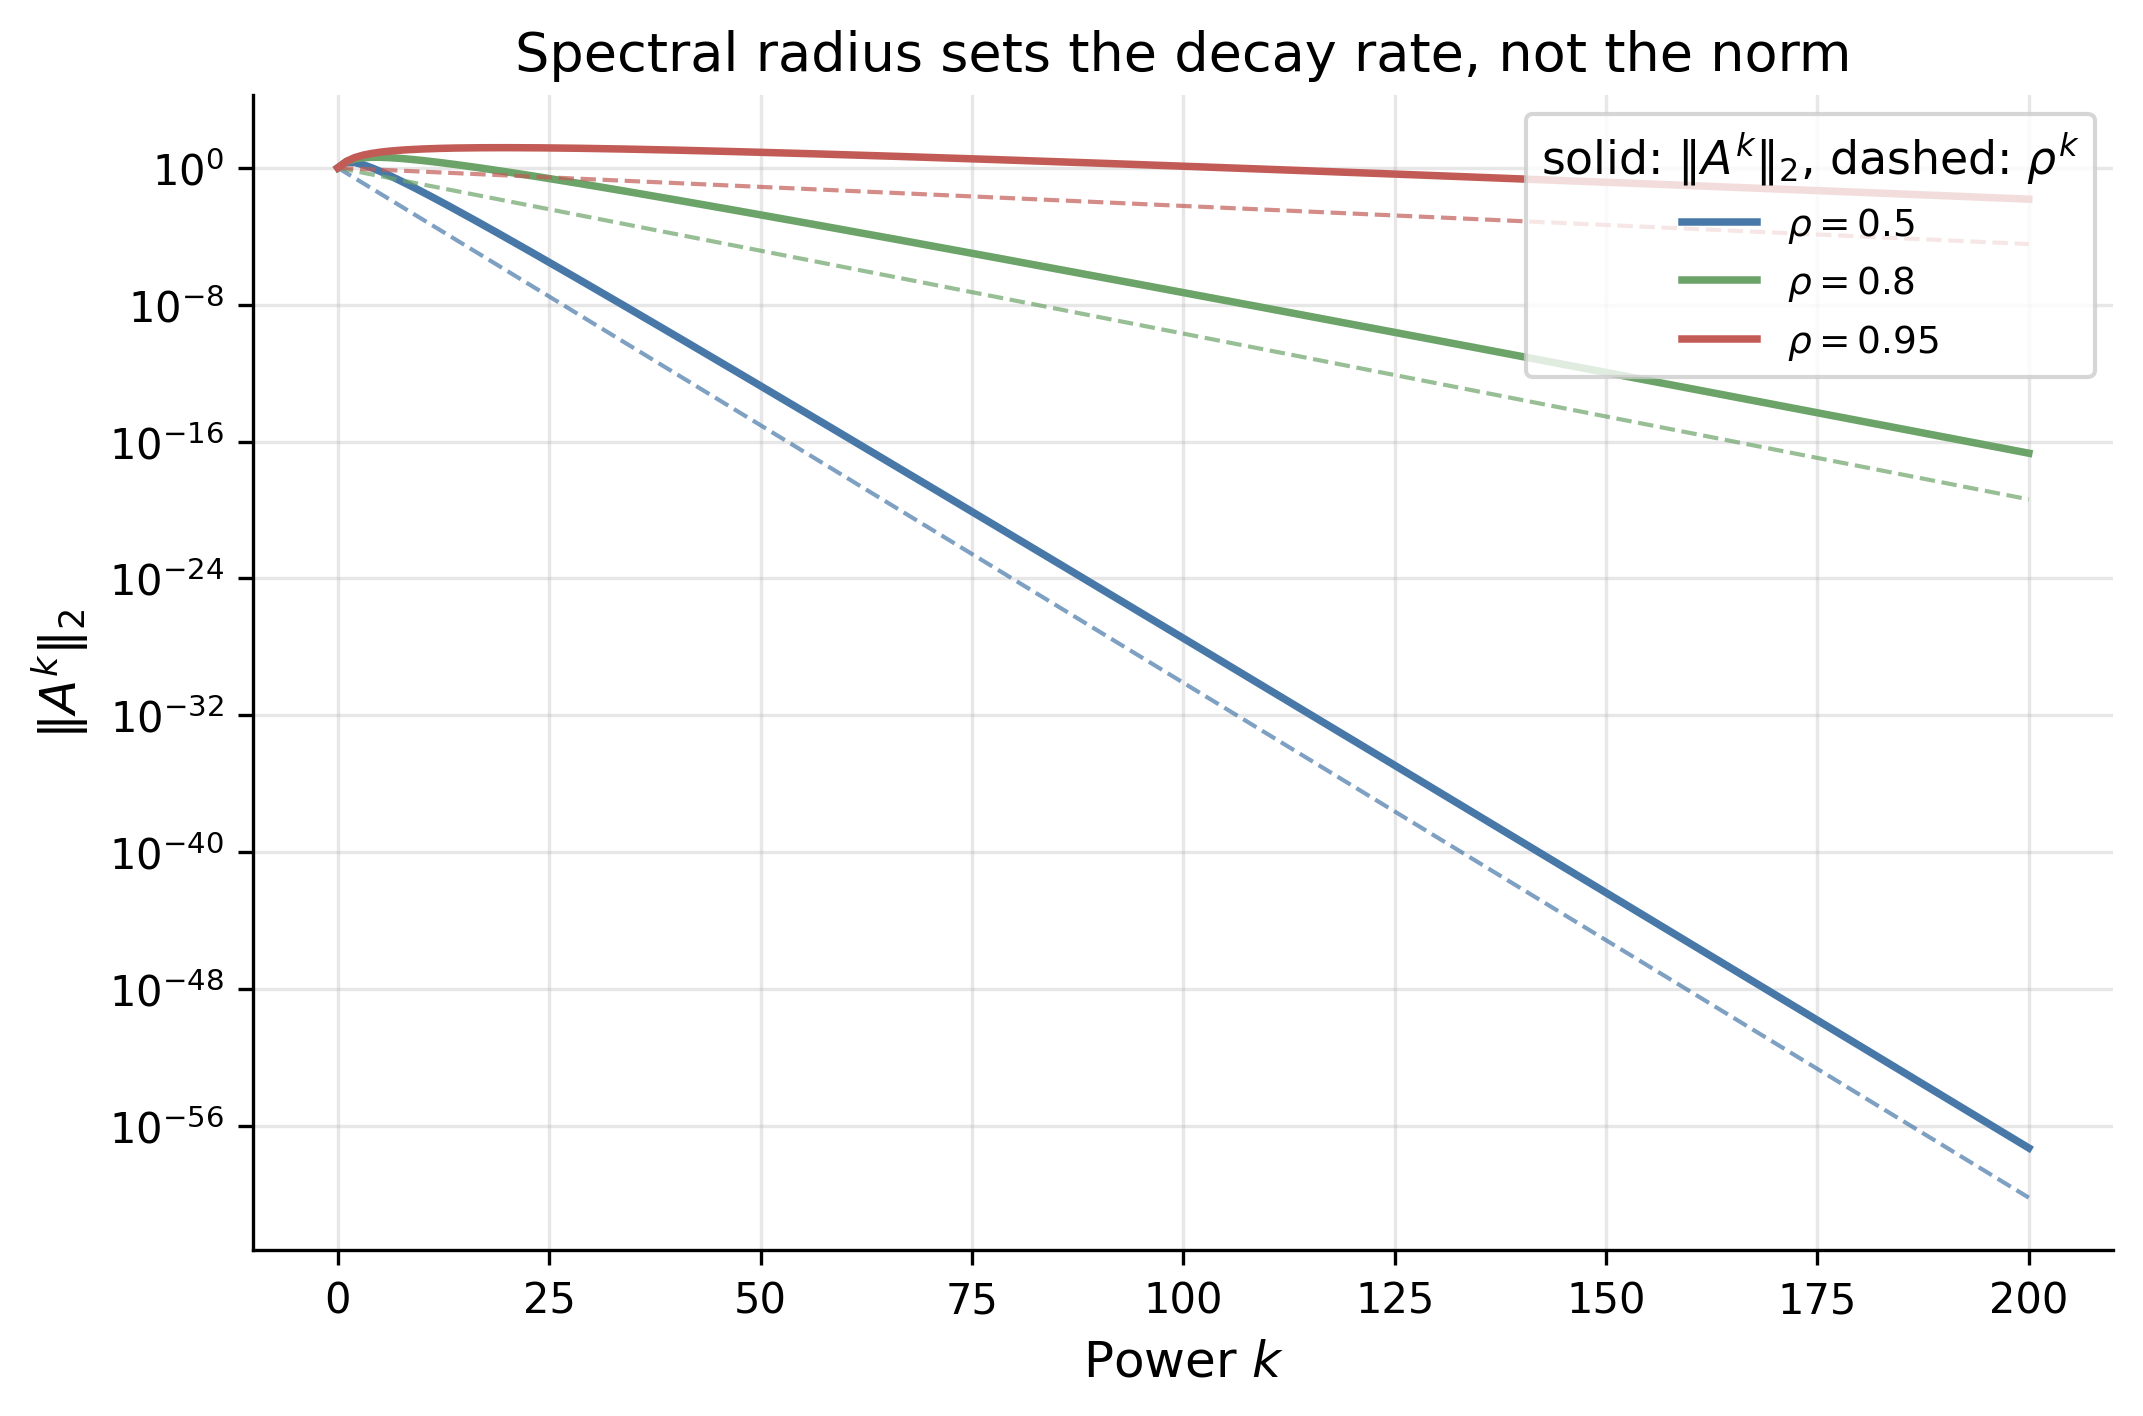
\includegraphics[width=0.78\textwidth]{../appA_preliminaries/sims/spectral_radius.png}
\caption{Operator norm $\|A^k\|_2$ of the powers of the non-normal matrix $A = \left[\begin{smallmatrix} \rho & 2 \\ 0 & \rho \end{smallmatrix}\right]$, on a log scale. The solid curves grow to a transient peak before decaying. The dashed curves are $\rho^k$. Both share the asymptotic slope, so $\rho$ sets the decay rate even though $\|A\|_2 > 1$.}
\label{fig:prelim_spectral}
\end{figure}

\begin{table}[h]
\centering
\caption{Powers of the non-normal matrix $A = \left[\begin{smallmatrix} \rho & 2 \\ 0 & \rho \end{smallmatrix}\right]$. The operator norm exceeds $\rho$ and the powers first grow, yet they decay asymptotically at rate $\rho$. The tail decay ratio $\|A^{k+1}\|/\|A^k\|$ approaches $\rho$ from above, with a benign $+O(1/k)$ finite-sample bias.}
\label{tab:prelim_spectral_radius}
\begin{tabular}{ccccc}
\hline
$\rho(A)$ & $\|A\|_2$ & Transient peak & at $k$ & Tail decay ratio \\
\hline
0.5 & 2.118 & 2.12 & 1 & 0.5027 \\
0.8 & 2.281 & 4.14 & 4 & 0.8043 \\
0.95 & 2.379 & 15.10 & 19 & 0.9552 \\
\hline
\end{tabular}
\end{table}


\subsubsection{The Neumann Series and the Resolvent}

\begin{theorem}[Neumann series, \citet{hornjohnson2013}]
\label{thm:prelim_neumann}
Let $P$ be a row-stochastic matrix and $\gamma \in [0, 1)$. Then $I - \gamma P$ is invertible and
\begin{equation}
(I - \gamma P)^{-1} = \sum_{m=0}^{\infty} (\gamma P)^m,
\label{eq:prelim_neumann}
\end{equation}
with the truncation error of the first $M{+}1$ terms bounded, in the supremum operator norm, by
\begin{equation}
\Bigl\| (I - \gamma P)^{-1} - \sum_{m=0}^{M} (\gamma P)^m \Bigr\|_\infty \leq \frac{\gamma^{M+1}}{1 - \gamma}.
\label{eq:prelim_neumann_bound}
\end{equation}
\end{theorem}

\begin{proof}
The plan is to telescope the partial sum, solve for the inverse, and bound the leftover with the geometric series. A row-stochastic $P$ has $\|P\|_\infty = 1$, so $\|(\gamma P)^m\|_\infty \leq \gamma^m$.\footnote{The \emph{supremum operator norm} $\|B\|_\infty = \max_i \sum_j |B_{ij}|$ is the largest absolute row sum. A row-stochastic matrix has every row summing to $1$, so $\|P\|_\infty = 1$, and averaging can never enlarge the biggest coordinate.} Multiply the partial sum by $I - \gamma P$ and let the terms cancel in pairs,
\begin{align*}
(I - \gamma P) \sum_{m=0}^{M} (\gamma P)^m = I - (\gamma P)^{M+1} && \text{(telescoping sum).}
\end{align*}
Because $\|(\gamma P)^{M+1}\|_\infty \leq \gamma^{M+1} \to 0$, the right side tends to $I$, so the partial sums converge and their limit is a genuine inverse, which is~\eqref{eq:prelim_neumann}. Solving the telescoped identity for the inverse and subtracting gives the leftover,
\begin{align*}
(I - \gamma P)^{-1} - \sum_{m=0}^{M} (\gamma P)^m = (I - \gamma P)^{-1} (\gamma P)^{M+1}.
\end{align*}
Taking norms and using $\|(I - \gamma P)^{-1}\|_\infty = \bigl\| \sum_m (\gamma P)^m \bigr\|_\infty \leq \sum_m \gamma^m = 1/(1-\gamma)$,
\begin{align*}
\Bigl\| (I - \gamma P)^{-1} - \sum_{m=0}^{M} (\gamma P)^m \Bigr\|_\infty
  &\leq \|(I - \gamma P)^{-1}\|_\infty\, \|(\gamma P)^{M+1}\|_\infty && \text{(submultiplicativity)} \\
  &\leq \frac{1}{1-\gamma} \cdot \gamma^{M+1} && \text{(the two bounds above),}
\end{align*}
which is~\eqref{eq:prelim_neumann_bound}.
\end{proof}

This identity is why the value function is a discounted sum of rewards.\footnote{The resolvent $(I - \gamma P^\pi)^{-1}$ is the policy-evaluation solve $V = (I - \gamma P^\pi)^{-1} r^\pi$ of Section~\ref{sec:planning_learning} and the fixed-policy value of Section~\ref{section:dist_robust_constrained}. Truncating the series is the same as truncating the planning horizon.} The exact value $V = (I - \gamma P^\pi)^{-1} r^\pi$ equals $\sum_m \gamma^m (P^\pi)^m r^\pi$, the expected discounted return. Truncating at $M$ terms is a finite-horizon approximation, and~\eqref{eq:prelim_neumann_bound} says the error falls at rate $\gamma$. Figure~\ref{fig:prelim_neumann} confirms this decay, and Table~\ref{tab:prelim_neumann} reports the terms needed for a fixed accuracy.

\begin{figure}[t]
\centering
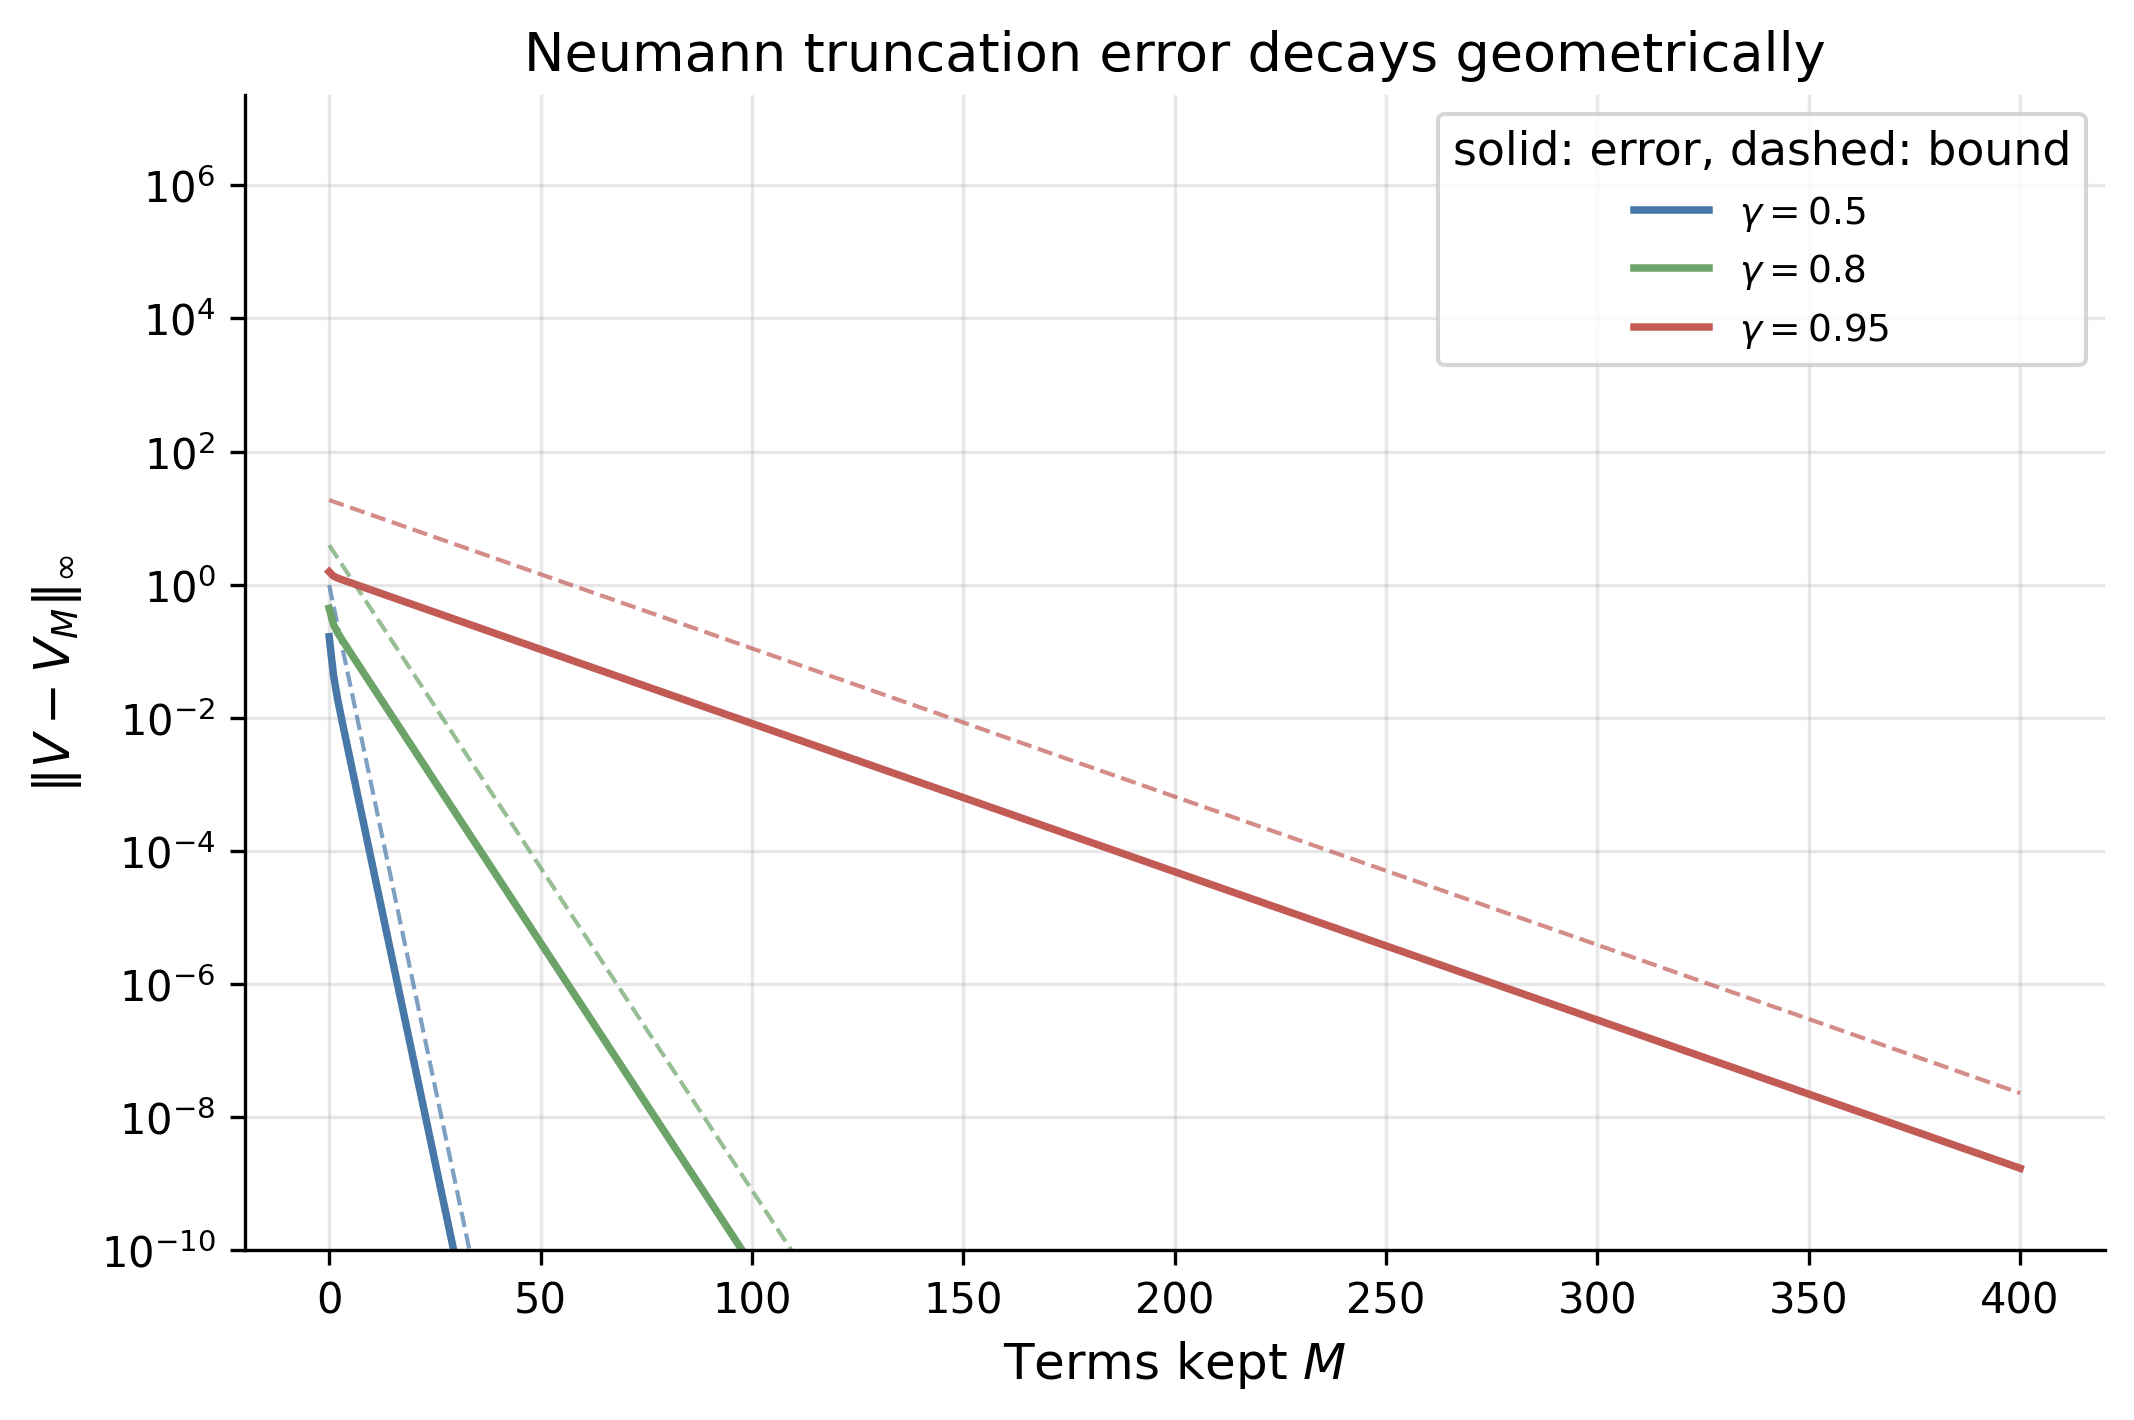
\includegraphics[width=0.78\textwidth]{../appA_preliminaries/sims/neumann_series.png}
\caption{Supremum-norm error of truncating $V = \sum_m \gamma^m P^m r$ at $M$ terms, on random 40-state chains, averaged over 30 seeds, on a log scale. The solid curves show the measured error and the dashed curves the bound $\gamma^{M+1}\|r\|_\infty/(1-\gamma)$ of Theorem~\ref{thm:prelim_neumann}.}
\label{fig:prelim_neumann}
\end{figure}

\begin{table}[h]
\centering
\caption{Truncating the Neumann series $V = \sum_m \gamma^m P^m r$ at $M$ terms, on random 40-state chains. The error falls at rate $\gamma$, matching the bound $\gamma^{M+1}\|r\|_\infty/(1-\gamma)$. Terms needed to reach $10^{-6}$, measured and predicted from the bound.}
\label{tab:prelim_neumann}
\begin{tabular}{ccc}
\hline
$\gamma$ & Terms to $10^{-6}$ & Predicted \\
\hline
0.5 & 17 & 20 \\
0.8 & 57 & 68 \\
0.95 & 276 & 326 \\
\hline
\end{tabular}
\end{table}


\subsubsection{The Stationary Distribution of a Markov Chain}

\begin{theorem}[Perron-Frobenius and mixing, \citet{levinperes2017}]
\label{thm:prelim_markov}
Let $P$ be the transition matrix of an irreducible, aperiodic Markov chain on a finite state space.\footnote{\emph{Irreducible} means every state can eventually reach every other state. \emph{Aperiodic} means the chain does not cycle with a fixed period. Together they make the chain \emph{primitive}: some power $P^k$ has all entries positive.} Then $P$ has a unique stationary distribution $d^\star$, meaning $d^\star P = d^\star$ with $d^\star \geq 0$ and $\sum_s d^\star_s = 1$. For every initial distribution $d_0$, the iterates $d_k = d_0 P^k$ converge to $d^\star$, and the total-variation distance obeys
\begin{equation}
\| d_0 P^k - d^\star \|_{\mathrm{TV}} \leq C\, |\lambda_2|^k,
\label{eq:prelim_markov_rate}
\end{equation}
where $\lambda_2$ is the second-largest eigenvalue in modulus and $C$ depends on the chain.
\end{theorem}

\begin{proof}
The plan is to expand the state distribution in the eigenbasis of $P$, so that the eigenvalue-$1$ term is the stationary distribution and every other term decays at its own eigenvalue. The Perron-Frobenius theorem for a primitive $P$ supplies the spectral picture.\footnote{For a primitive stochastic matrix the Perron-Frobenius theorem states that $1$ is an eigenvalue, it is simple (a one-dimensional eigenspace), and every other eigenvalue has modulus strictly less than $1$. The left eigenvector for eigenvalue $1$, normalized to sum to one, is the stationary distribution $d^\star$. See \citet{levinperes2017} for the general case, including the coupling proof that removes the diagonalizability assumption used here.} The right eigenvector for eigenvalue $1$ is the all-ones vector, since $P \mathbf{1} = \mathbf{1}$ by row-stochasticity, and the matching left eigenvector is $d^\star$. Assume $P$ is diagonalizable with left eigenvectors $w_1 = d^\star, w_2, \ldots$ and eigenvalues $1 = \lambda_1 > |\lambda_2| \geq \cdots$. Expand the initial distribution and push it through $k$ steps,
\begin{align*}
d_0 P^k = \sum_i c_i \lambda_i^k w_i
  &= \underbrace{c_1 w_1}_{= \, d^\star} + \sum_{i \geq 2} c_i \lambda_i^k w_i && \text{(eigen-expansion, $\lambda_1 = 1$).}
\end{align*}
The leading coefficient is $c_1 = 1$, because $d_0$ and $d^\star$ are both probability vectors and the eigenvalue-$1$ component of any distribution is $d^\star$. Subtracting it,
\begin{align*}
\| d_0 P^k - d^\star \|_{\mathrm{TV}} = \Bigl\| \sum_{i \geq 2} c_i \lambda_i^k w_i \Bigr\|_{\mathrm{TV}}
  &\leq \Bigl( \sum_{i \geq 2} |c_i|\, \|w_i\|_{\mathrm{TV}} \Bigr) |\lambda_2|^k && \text{($|\lambda_i| \leq |\lambda_2|$).}
\end{align*}
Collecting the bracket into a constant $C$ gives~\eqref{eq:prelim_markov_rate}.
\end{proof}

This is the fact behind on-policy sampling.\footnote{The stationary distribution $d^\pi$ is the sampling distribution under which the projected Bellman operator contracts (Section~\ref{sec:planning_learning}), the ergodic distribution of the exogenous and heterogeneous-agent chains of Section~\ref{section:rl_macro}, and the state occupancy that model-based rollouts must respect (Section~\ref{section:world_models}). The mixing rate $1 - |\lambda_2|$ sets how fast a simulated chain forgets its start.} Figure~\ref{fig:prelim_markov} runs the power iteration $d_k = d_0 P^k$ for chains with three mixing speeds. The total-variation distance falls at rate $|\lambda_2|$, and slower-mixing chains take proportionally longer to forget the start (Table~\ref{tab:prelim_markov}).

\begin{figure}[t]
\centering
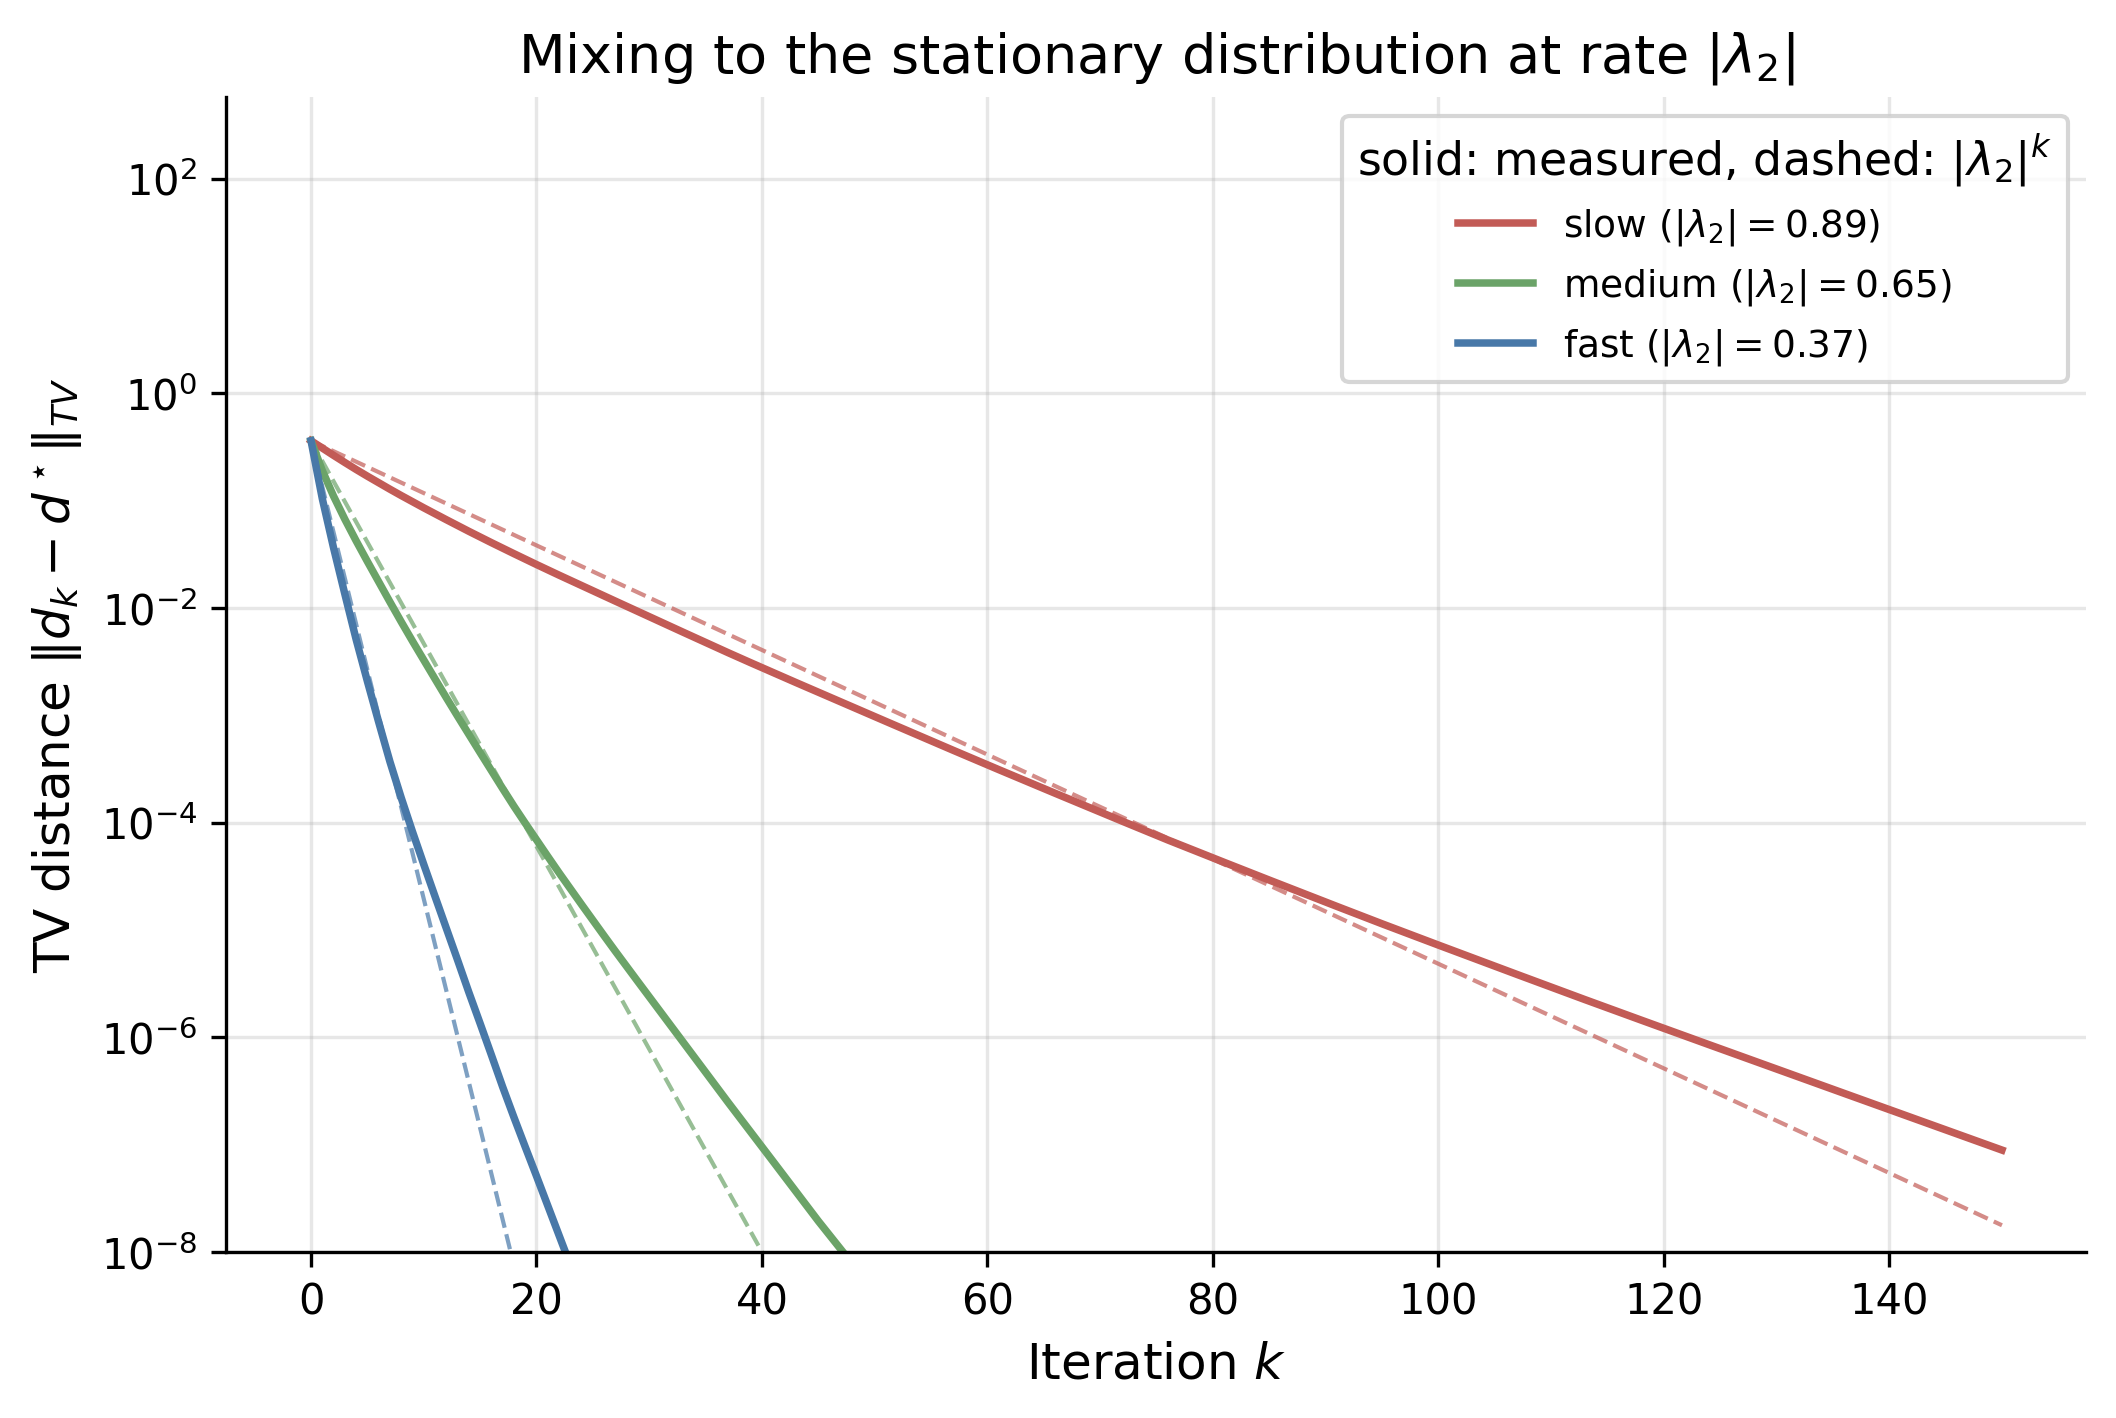
\includegraphics[width=0.78\textwidth]{../appA_preliminaries/sims/markov_stationary.png}
\caption{Total-variation distance $\|d_k - d^\star\|_{\mathrm{TV}}$ of the state distribution $d_k = d_0 P^k$ from the stationary distribution, on random 8-state chains at three mixing speeds, averaged over 30 seeds, on a log scale. The solid curves show the measured distance and the dashed curves the $|\lambda_2|^k$ rate of Theorem~\ref{thm:prelim_markov}.}
\label{fig:prelim_markov}
\end{figure}

\begin{table}[h]
\centering
\caption{Convergence of the state distribution $d_k = d_0 P^k$ to the stationary distribution $d^\star$ on random 8-state chains, at three mixing speeds. The total-variation distance falls at rate $|\lambda_2|$, the second-largest eigenvalue modulus. The residual confirms $d^\star P = d^\star$. Means over 30 seeds.}
\label{tab:prelim_markov}
\begin{tabular}{lccc}
\hline
Chain & $|\lambda_2|$ & $\|d^\star P - d^\star\|_\infty$ & Iters to $10^{-6}$ \\
\hline
slow & 0.8939 & 2.2e-16 & 123 \\
medium & 0.6473 & 2.5e-16 & 33 \\
fast & 0.3742 & 2.2e-16 & 16 \\
\hline
\end{tabular}
\end{table}


\subsubsection{Orthogonal Projection is Nonexpansive}

\begin{theorem}[Projection geometry, \citet{luenberger1969}]
\label{thm:prelim_hilbert}
Let $H$ be an inner-product space, let $M \subseteq H$ be a closed subspace, and let $\Pi$ be the orthogonal projection onto $M$.\footnote{The \emph{orthogonal projection} $\Pi x$ is the point of $M$ closest to $x$. Its defining property is that the residual $x - \Pi x$ is orthogonal to every vector in $M$, written $x - \Pi x \perp M$.} Then for every $x \in H$ the Pythagorean identity
\begin{equation}
\|x\|^2 = \|\Pi x\|^2 + \|x - \Pi x\|^2
\label{eq:prelim_pythagoras}
\end{equation}
holds, and consequently $\Pi$ is nonexpansive, $\|\Pi x - \Pi y\| \leq \|x - y\|$.
\end{theorem}

\begin{proof}
The plan is to split $x$ into its projection and its residual, use that the two are orthogonal, and expand the squared norm. By definition $\Pi x \in M$ and the residual satisfies $x - \Pi x \perp M$, so in particular the two pieces are orthogonal and $\langle \Pi x, x - \Pi x \rangle = 0$. Write $x$ as their sum and expand,
\begin{align*}
\|x\|^2 = \|\Pi x + (x - \Pi x)\|^2
  &= \|\Pi x\|^2 + 2 \langle \Pi x, x - \Pi x \rangle + \|x - \Pi x\|^2 && \text{(expand the square)} \\
  &= \|\Pi x\|^2 + \|x - \Pi x\|^2 && \text{(orthogonality kills the cross term),}
\end{align*}
which is~\eqref{eq:prelim_pythagoras}. Since $\|x - \Pi x\|^2 \geq 0$, dropping it gives $\|\Pi x\|^2 \leq \|x\|^2$, so $\|\Pi x\| \leq \|x\|$. Projection is linear, so applying this to $x - y$ gives $\|\Pi x - \Pi y\| = \|\Pi(x - y)\| \leq \|x - y\|$, which is nonexpansiveness.\footnote{The Cauchy-Schwarz inequality $|\langle a, b \rangle| \leq \|a\|\,\|b\|$ is the same statement in disguise. It says the projection of $a$ onto the line through $b$ is no longer than $a$ itself.}
\end{proof}

Nonexpansiveness is what keeps linear function approximation stable.\footnote{Composing the nonexpansive $\Pi$ with the $\gamma$-contraction $T^\pi$ gives the projected Bellman operator $\Pi T^\pi$, a $\gamma$-contraction whose fixed point is the temporal-difference solution (Section~\ref{sec:planning_learning}). When sampling is off-policy the projection is oblique rather than orthogonal, it can lengthen vectors, and the contraction can fail.} Under on-policy sampling the projection onto the space of representable value functions cannot lengthen a vector, so the projected Bellman operator remains a contraction. Figure~\ref{fig:prelim_hilbert} draws the geometry, and Table~\ref{tab:prelim_hilbert} checks the identity numerically.

\begin{figure}[t]
\centering
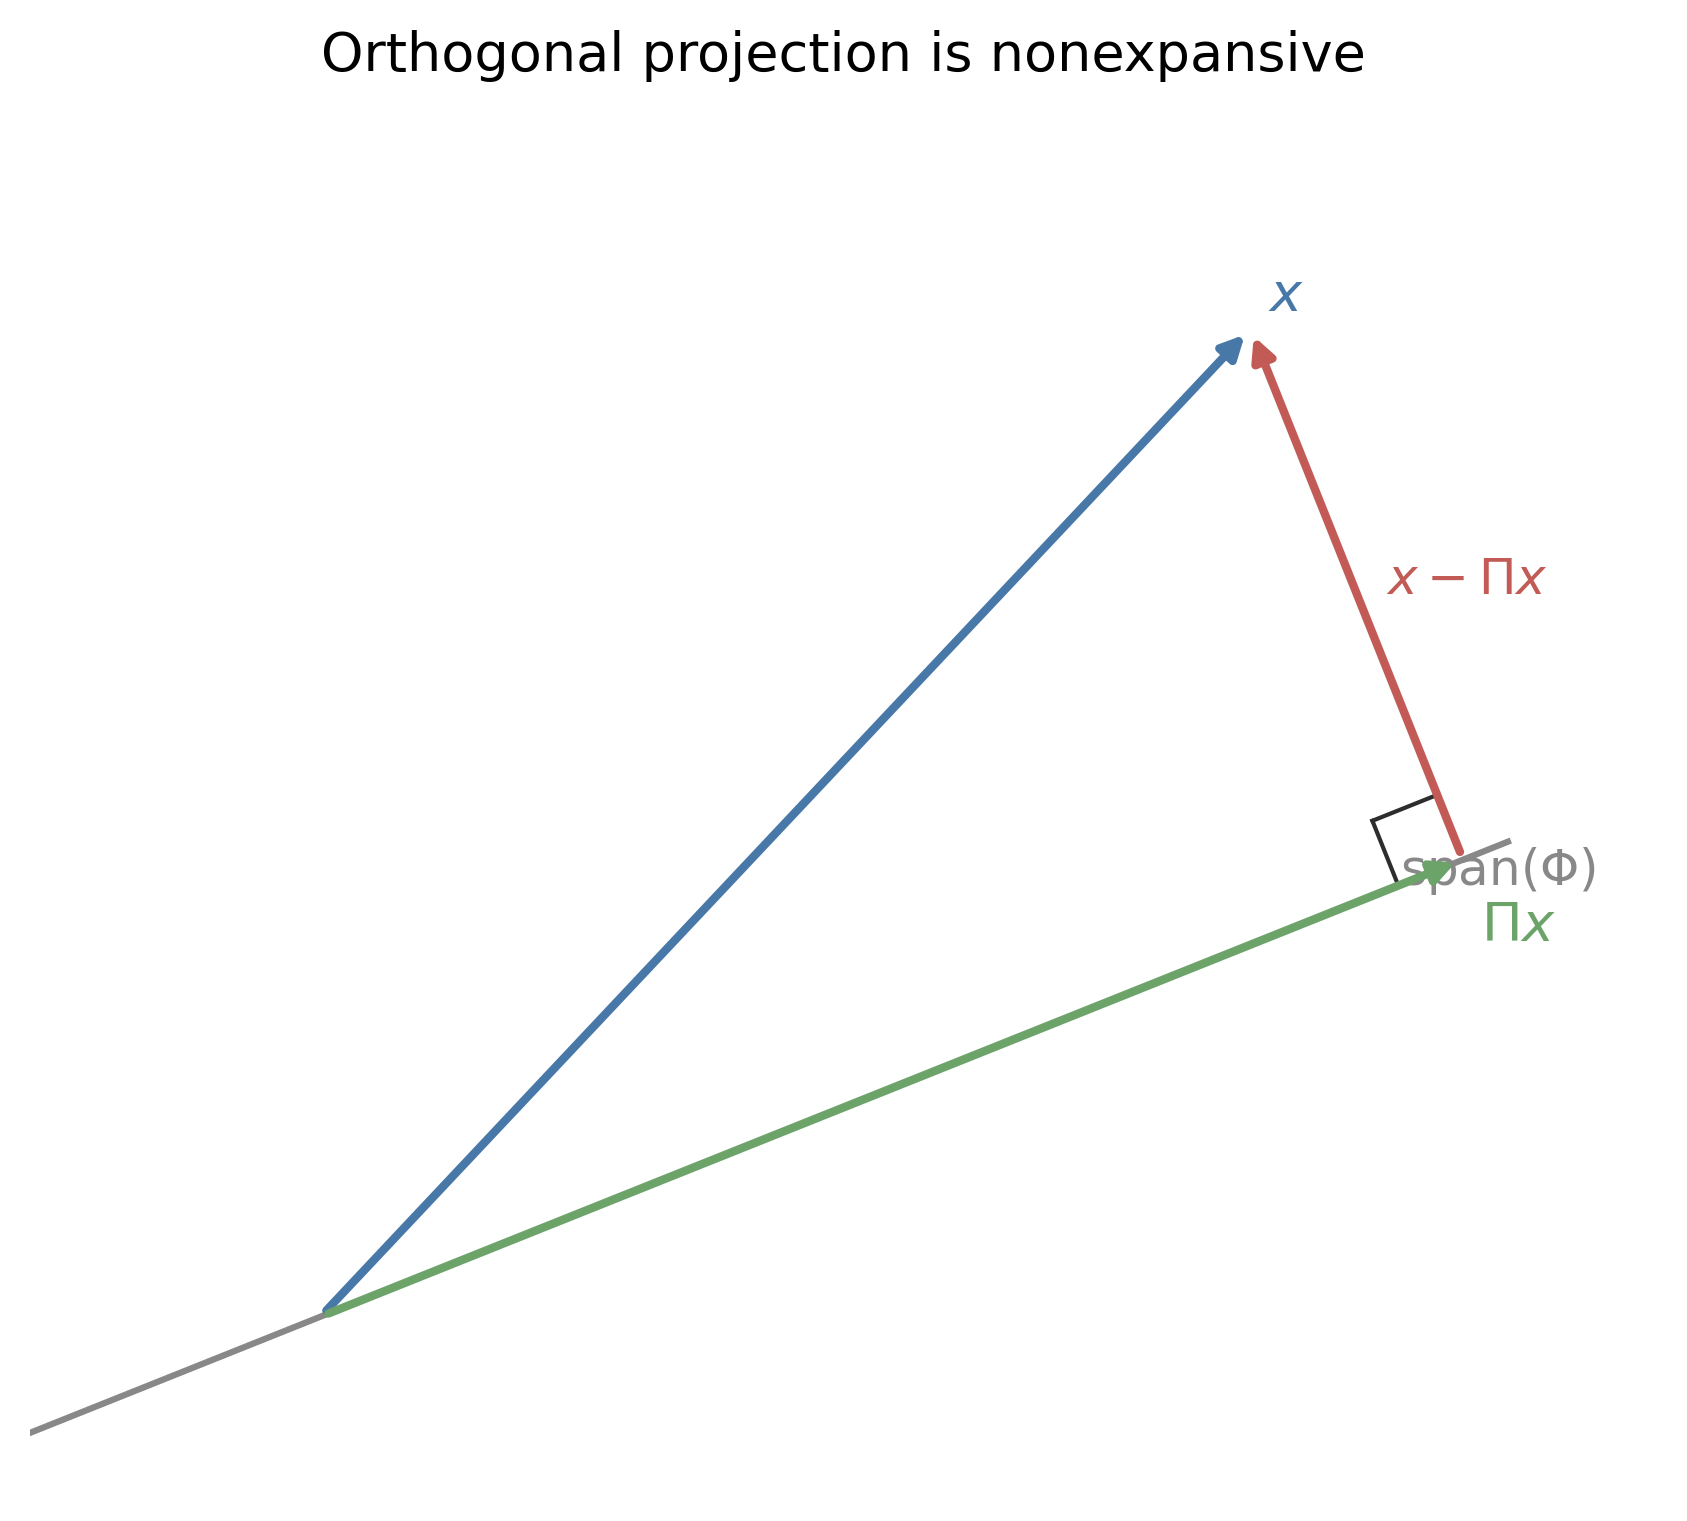
\includegraphics[width=0.5\textwidth]{../appA_preliminaries/sims/hilbert_projection.png}
\caption{The orthogonal projection $\Pi x$ of a point $x$ onto a subspace. The residual $x - \Pi x$ meets the subspace at a right angle, so the three vectors form a right triangle and $\Pi x$ is a leg no longer than the hypotenuse $x$.}
\label{fig:prelim_hilbert}
\end{figure}

\begin{table}[h]
\centering
\caption{Numeric check of the Pythagorean identity and nonexpansiveness for the point and subspace drawn in Figure~\ref{fig:prelim_hilbert}. The squared lengths add exactly, and the projection is no longer than the original.}
\label{tab:prelim_hilbert}
\begin{tabular}{lc}
\hline
Quantity & Value \\
\hline
$\|x\|^2$ & 5.4500 \\
$\|\Pi x\|^2 + \|x - \Pi x\|^2$ & 5.4500 \\
$\|\Pi x\|$ & 2.1169 \\
$\|x\|$ & 2.3345 \\
\hline
\end{tabular}
\end{table}


\subsection{Probability}
\label{prelim:probability}

Reinforcement learning estimates expectations from samples and then acts on them. Three probability facts make that safe. The first says a nonlinear objective and an expectation do not commute, and fixes the direction of the error. The second says a sample average converges to the mean it estimates, and quantifies the fluctuation around it. The third says a sequence of running estimates that drifts the right way in conditional mean settles down almost surely, the tool that turns a single noisy trajectory into a convergence proof.

\subsubsection{Jensen's Inequality}

\begin{theorem}[Jensen's inequality, \citet{durrett}]
\label{thm:prelim_jensen}
Let $\varphi : \mathbb{R} \to \mathbb{R}$ be convex and let $X$ be an integrable random variable with $\varphi(X)$ also integrable.\footnote{A function $\varphi$ is \emph{convex} if its graph lies on or below every chord, equivalently $\varphi(\lambda x + (1-\lambda) y) \leq \lambda \varphi(x) + (1-\lambda)\varphi(y)$ for $\lambda \in [0,1]$. \emph{Integrable} means the expectation $\mathbb{E}[X]$ is finite.} Then
\begin{equation}
\varphi\bigl(\mathbb{E}[X]\bigr) \leq \mathbb{E}\bigl[\varphi(X)\bigr].
\label{eq:prelim_jensen}
\end{equation}
The inequality reverses when $\varphi$ is concave, and holds with equality when $\varphi$ is affine.
\end{theorem}

\begin{proof}
The plan is to trap $\varphi$ below by a straight line that touches it at the mean, then take expectations so the linear part collapses. Write $m = \mathbb{E}[X]$. A convex function has a supporting line at every point, so there is a slope $c$ with $\varphi(x) \geq \varphi(m) + c\,(x - m)$ for all $x$.\footnote{A \emph{supporting line} at $m$ is a line through $(m, \varphi(m))$ that stays weakly below the graph. For a differentiable $\varphi$ it is the tangent, $c = \varphi'(m)$; in general $c$ is any \emph{subgradient}, and convexity guarantees at least one exists.} Evaluate this at $x = X$ and take expectations,
\begin{align*}
\mathbb{E}[\varphi(X)]
  &\geq \varphi(m) + c\,\mathbb{E}[X - m] && \text{(supporting line at $m$, then linearity)} \\
  &= \varphi(m) + c \cdot 0 = \varphi(\mathbb{E}[X]) && \text{($\mathbb{E}[X] = m$),}
\end{align*}
which is~\eqref{eq:prelim_jensen}. The concave case applies this to $-\varphi$, and an affine $\varphi$ meets its own supporting line everywhere, so the inequality is an equality.
\end{proof}

Jensen's inequality is why an expectation and a nonlinear objective cannot be swapped for free.\footnote{The convexity of the maximum drives the overestimation bias of Q-learning and its double-estimator corrections in Section~\ref{sec:planning_learning}, where the expected maximum of noisy action values exceeds the maximum of their means. The convexity of the exponential and of coherent risk measures supports the entropic-risk and distributionally robust value operators of Section~\ref{section:dist_robust_constrained}.} The clearest reinforcement-learning instance is the maximization bias. The maximum is a convex function, so the expected maximum of noisy action-value estimates sits above the maximum of their means, and a bootstrapped target that maximizes over sampled values overestimates. The same inequality, applied to the exponential, is behind the risk-sensitive and distributionally robust objectives that penalize the spread of returns. Figure~\ref{fig:prelim_jensen} estimates the gap for two convex functions, and Table~\ref{tab:prelim_jensen} confirms it matches the closed form and never turns negative.

\begin{figure}[t]
\centering
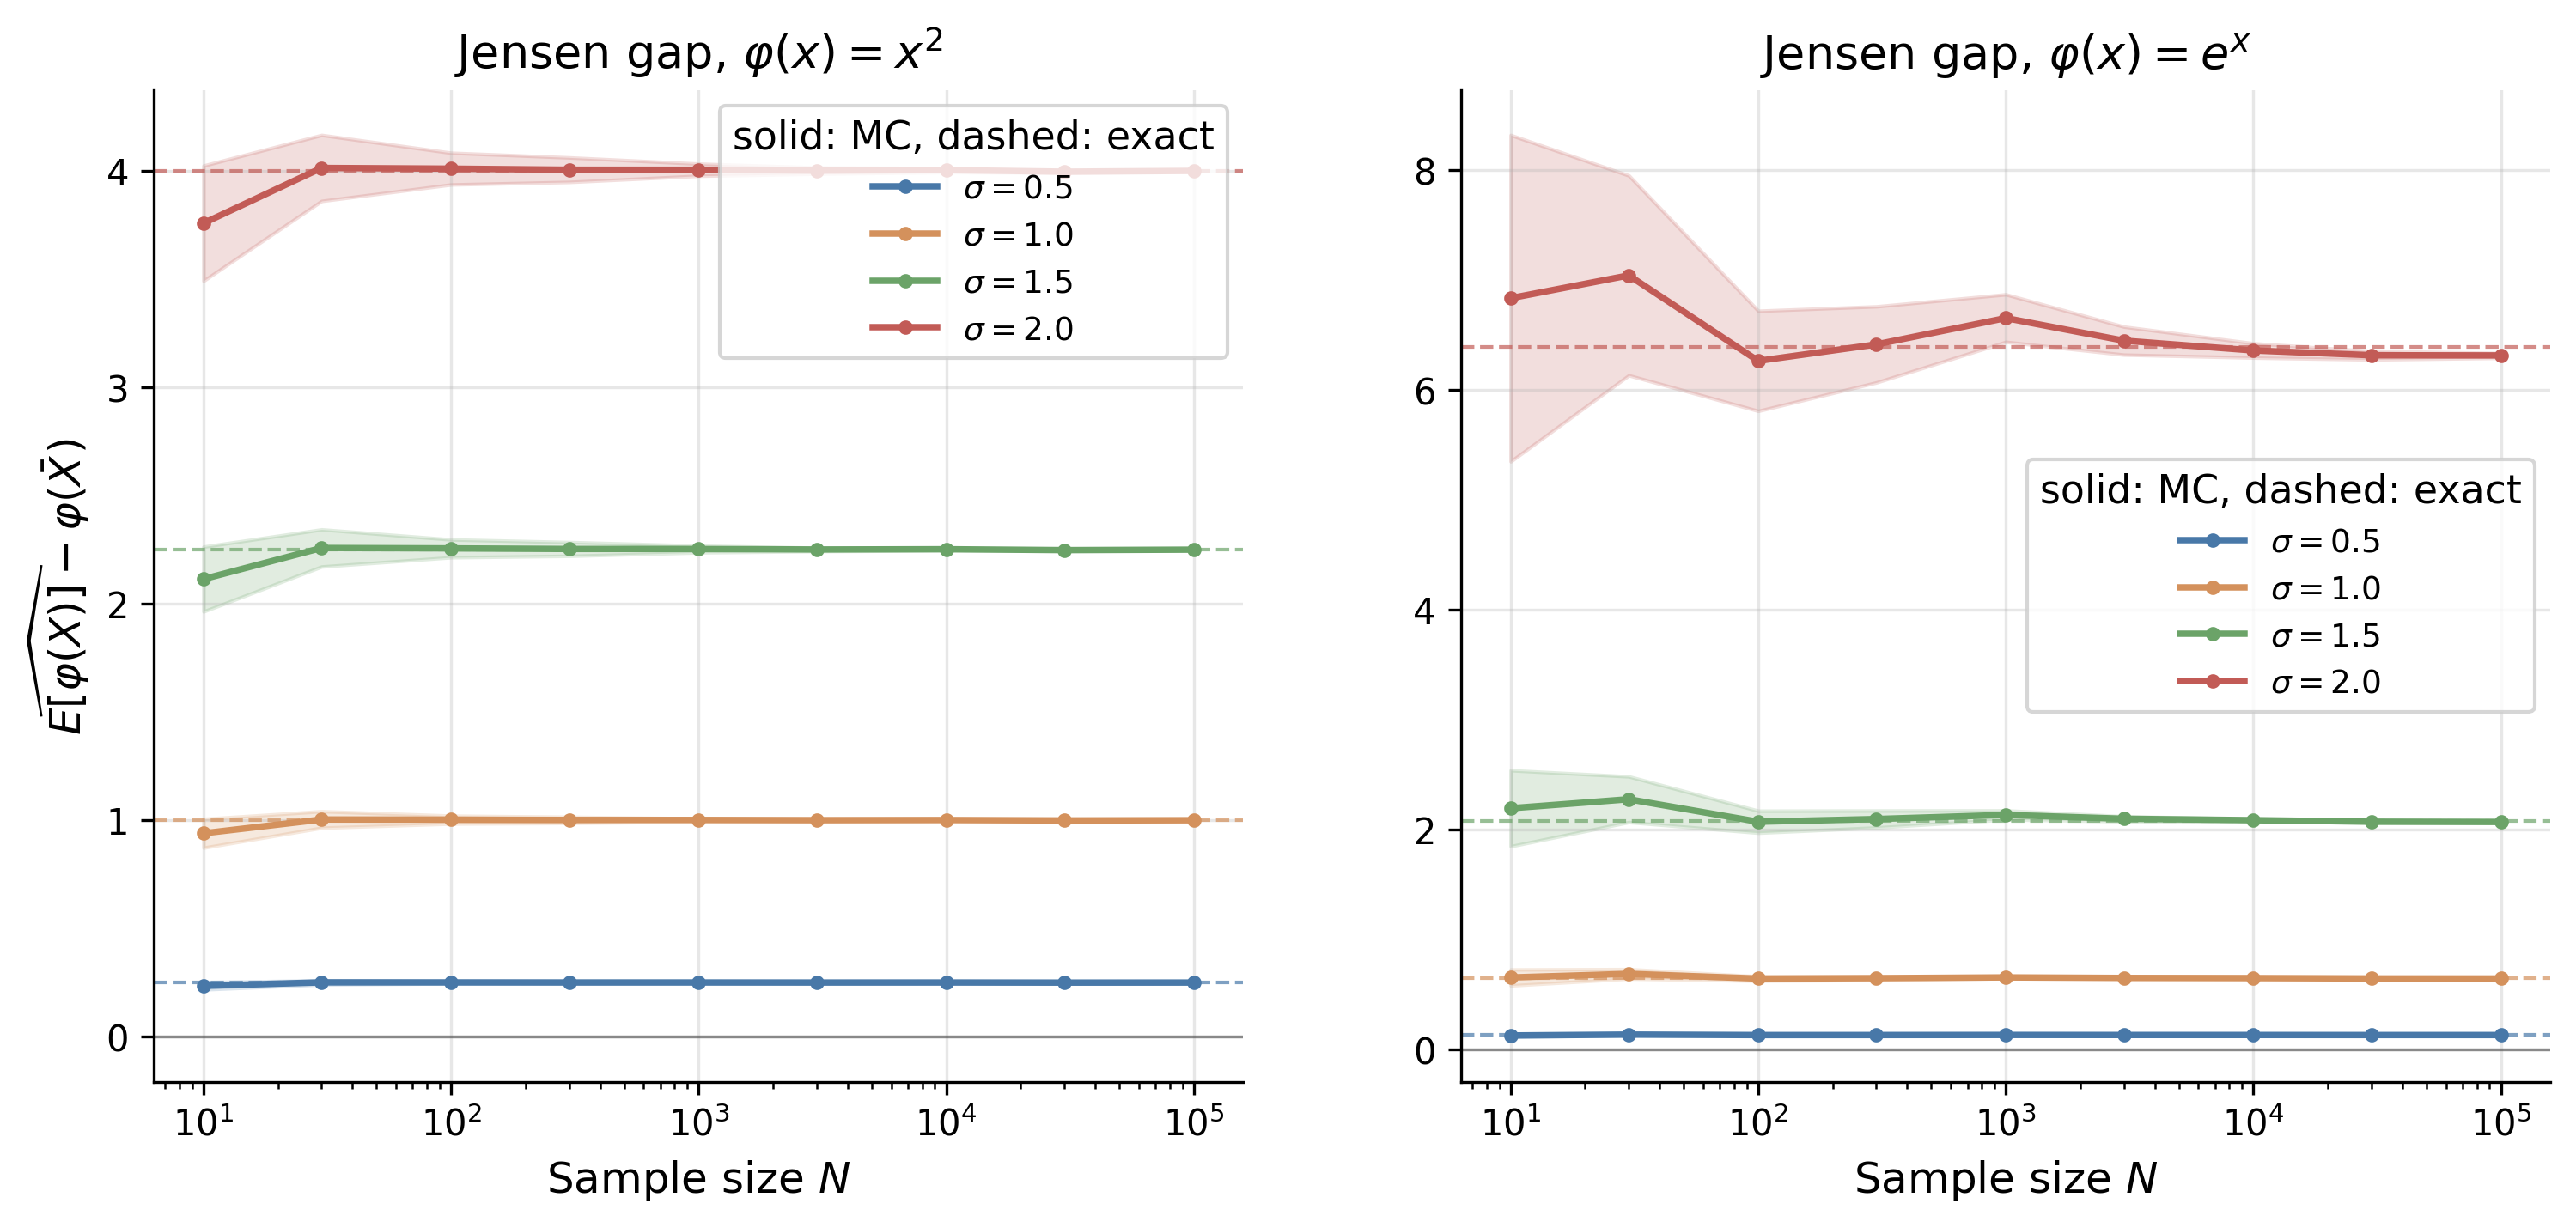
\includegraphics[width=0.95\textwidth]{../appA_preliminaries/sims/jensen_gap.png}
\caption{Plug-in Monte Carlo estimate of the Jensen gap $\mathbb{E}[\varphi(X)] - \varphi(\mathbb{E}[X])$ for $X \sim N(0, \sigma^2)$ against sample size $N$, for $\varphi(x) = x^2$ (left) and $\varphi(x) = e^x$ (right), at four values of $\sigma$, averaged over 40 seeds with a $\pm 1$ standard-error band. The dashed lines are the closed-form gaps $\sigma^2$ and $e^{\sigma^2/2} - 1$. The solid line at zero marks the sign floor the inequality forbids the gap to cross.}
\label{fig:prelim_jensen}
\end{figure}

\begin{table}[h]
\centering
\caption{Maximization bias for independent Gaussian action-value estimates, over 400000 Monte Carlo replicates per cell. With equal true action values the whole expected maximum is bias, and it equals $\sigma\,\mathbb{E}[\max_a Z_a]$ in closed form. The last column gives the bias once the best action is separated from the rest by one unit, at which point the maximum is nearly deterministic and the bias collapses.}
\label{tab:prelim_jensen}
\begin{tabular}{rrrrr}
\hline
actions & $\sigma$ & measured gap & $\sigma\,\mathbb{E}[\max_a Z_a]$ & bias at separation $1$ \\
\hline
2 & 0.25 & 0.1413 & 0.1409 & 0.0009 \\
2 & 1.00 & 0.5663 & 0.5637 & 0.2024 \\
8 & 0.25 & 0.3559 & 0.3558 & 0.0016 \\
8 & 1.00 & 1.4232 & 1.4233 & 0.6658 \\
32 & 0.25 & 0.5174 & 0.5171 & 0.0045 \\
32 & 1.00 & 2.0697 & 2.0684 & 1.1568 \\
\hline
\end{tabular}
\end{table}


\subsubsection{The Law of Large Numbers and the Central Limit Theorem}

\begin{theorem}[Law of large numbers and central limit theorem, \citet{durrett}]
\label{thm:prelim_lln_clt}
Let $X_1, X_2, \ldots$ be independent and identically distributed with mean $\mu = \mathbb{E}[X_1]$ and finite variance $\sigma^2 = \operatorname{Var}(X_1)$, and let $\bar X_n = \frac{1}{n}\sum_{i=1}^n X_i$ be the sample mean.\footnote{\emph{Independent and identically distributed} (i.i.d.) means the draws share one law and none informs any other. \emph{Almost surely} means with probability one, the strongest sense in which a sequence of random quantities can converge.} Then the sample mean converges to the population mean,
\begin{equation}
\bar X_n \to \mu \quad \text{almost surely} \qquad (\text{law of large numbers}),
\label{eq:prelim_lln}
\end{equation}
and its rescaled fluctuation converges in distribution to a Gaussian,
\begin{equation}
\sqrt{n}\,(\bar X_n - \mu) \;\Rightarrow\; N(0, \sigma^2) \qquad (\text{central limit theorem}),
\label{eq:prelim_clt}
\end{equation}
whatever the shape of the underlying distribution.\footnote{Convergence \emph{in distribution}, written $\Rightarrow$, means the cumulative distribution functions converge at every continuity point. It is a statement about the shape of the fluctuation, not about any single realization.}
\end{theorem}

\begin{proof}
The plan is to read the law of large numbers off Chebyshev's inequality, and the central limit theorem off a Taylor expansion of the characteristic function whose limit is the Gaussian transform. Independence makes the variance of the mean shrink, $\operatorname{Var}(\bar X_n) = \sigma^2/n$. Chebyshev's inequality then controls the deviation,
\begin{align*}
\mathbb{P}\bigl(|\bar X_n - \mu| \geq \varepsilon\bigr)
  &\leq \frac{\operatorname{Var}(\bar X_n)}{\varepsilon^2} = \frac{\sigma^2}{n\varepsilon^2} \to 0 && \text{(Chebyshev, independence),}
\end{align*}
which is convergence in probability.\footnote{This gives the \emph{weak} law. The \emph{strong} law~\eqref{eq:prelim_lln}, with almost-sure convergence, needs a Borel-Cantelli argument along a subsequence or Kolmogorov's criterion; see \citet{durrett}. The simulation below shows the stronger pathwise convergence.} For the central limit theorem standardize the summands, $Y_i = (X_i - \mu)/\sigma$, so $\mathbb{E}[Y_i] = 0$ and $\operatorname{Var}(Y_i) = 1$, and write $S_n = \frac{1}{\sqrt n}\sum_i Y_i = \sqrt{n}(\bar X_n - \mu)/\sigma$. Let $\psi(t) = \mathbb{E}[e^{itY_1}]$ be the characteristic function of a standardized summand, with $\psi(0) = 1$, $\psi'(0) = 0$, and $\psi''(0) = -1$. Expanding to second order and using independence,
\begin{align*}
\mathbb{E}\bigl[e^{it S_n}\bigr]
  &= \psi\!\left(\frac{t}{\sqrt n}\right)^{\! n} && \text{(i.i.d.\ factorization)} \\
  &= \left(1 - \frac{t^2}{2n} + o\!\left(\frac{1}{n}\right)\right)^{\! n} && \text{(Taylor expansion of $\psi$)} \\
  &\to e^{-t^2/2} && \text{($(1 + a/n)^n \to e^a$).}
\end{align*}
The limit $e^{-t^2/2}$ is the characteristic function of $N(0,1)$, so by the continuity theorem $S_n \Rightarrow N(0,1)$, and undoing the standardization gives $\sqrt{n}(\bar X_n - \mu) \Rightarrow N(0, \sigma^2)$, which is~\eqref{eq:prelim_clt}.
\end{proof}

These two results are why learning from samples works and how fast.\footnote{The $\sqrt{n}$ rate is the width of the bandit confidence bounds of Section~\ref{section:bandits}, the standard error attached to every Monte Carlo value estimate in Section~\ref{sec:planning_learning}, and the large-sample distribution of the simulation-based structural estimators of Section~\ref{section:rl_econ_models}.} The law of large numbers is the license to replace an expectation by a sample average, the operation underneath every Monte Carlo return estimate and every empirical Bellman backup. The central limit theorem fixes the price of doing so. The error shrinks at rate $1/\sqrt{n}$ and is asymptotically Gaussian, which is what turns a raw estimate into a confidence interval. Figure~\ref{fig:prelim_lln_clt} shows the sample mean of skewed exponential draws settling on its mean, and the rescaled fluctuation taking the Gaussian shape at a moderate sample size. Table~\ref{tab:prelim_lln_clt} checks that the variance of the rescaled mean matches $\sigma^2$ and that its skewness and excess kurtosis approach the normal values of zero across three non-normal sources, the discrete Bernoulli approaching more slowly through its lattice.

\begin{figure}[t]
\centering
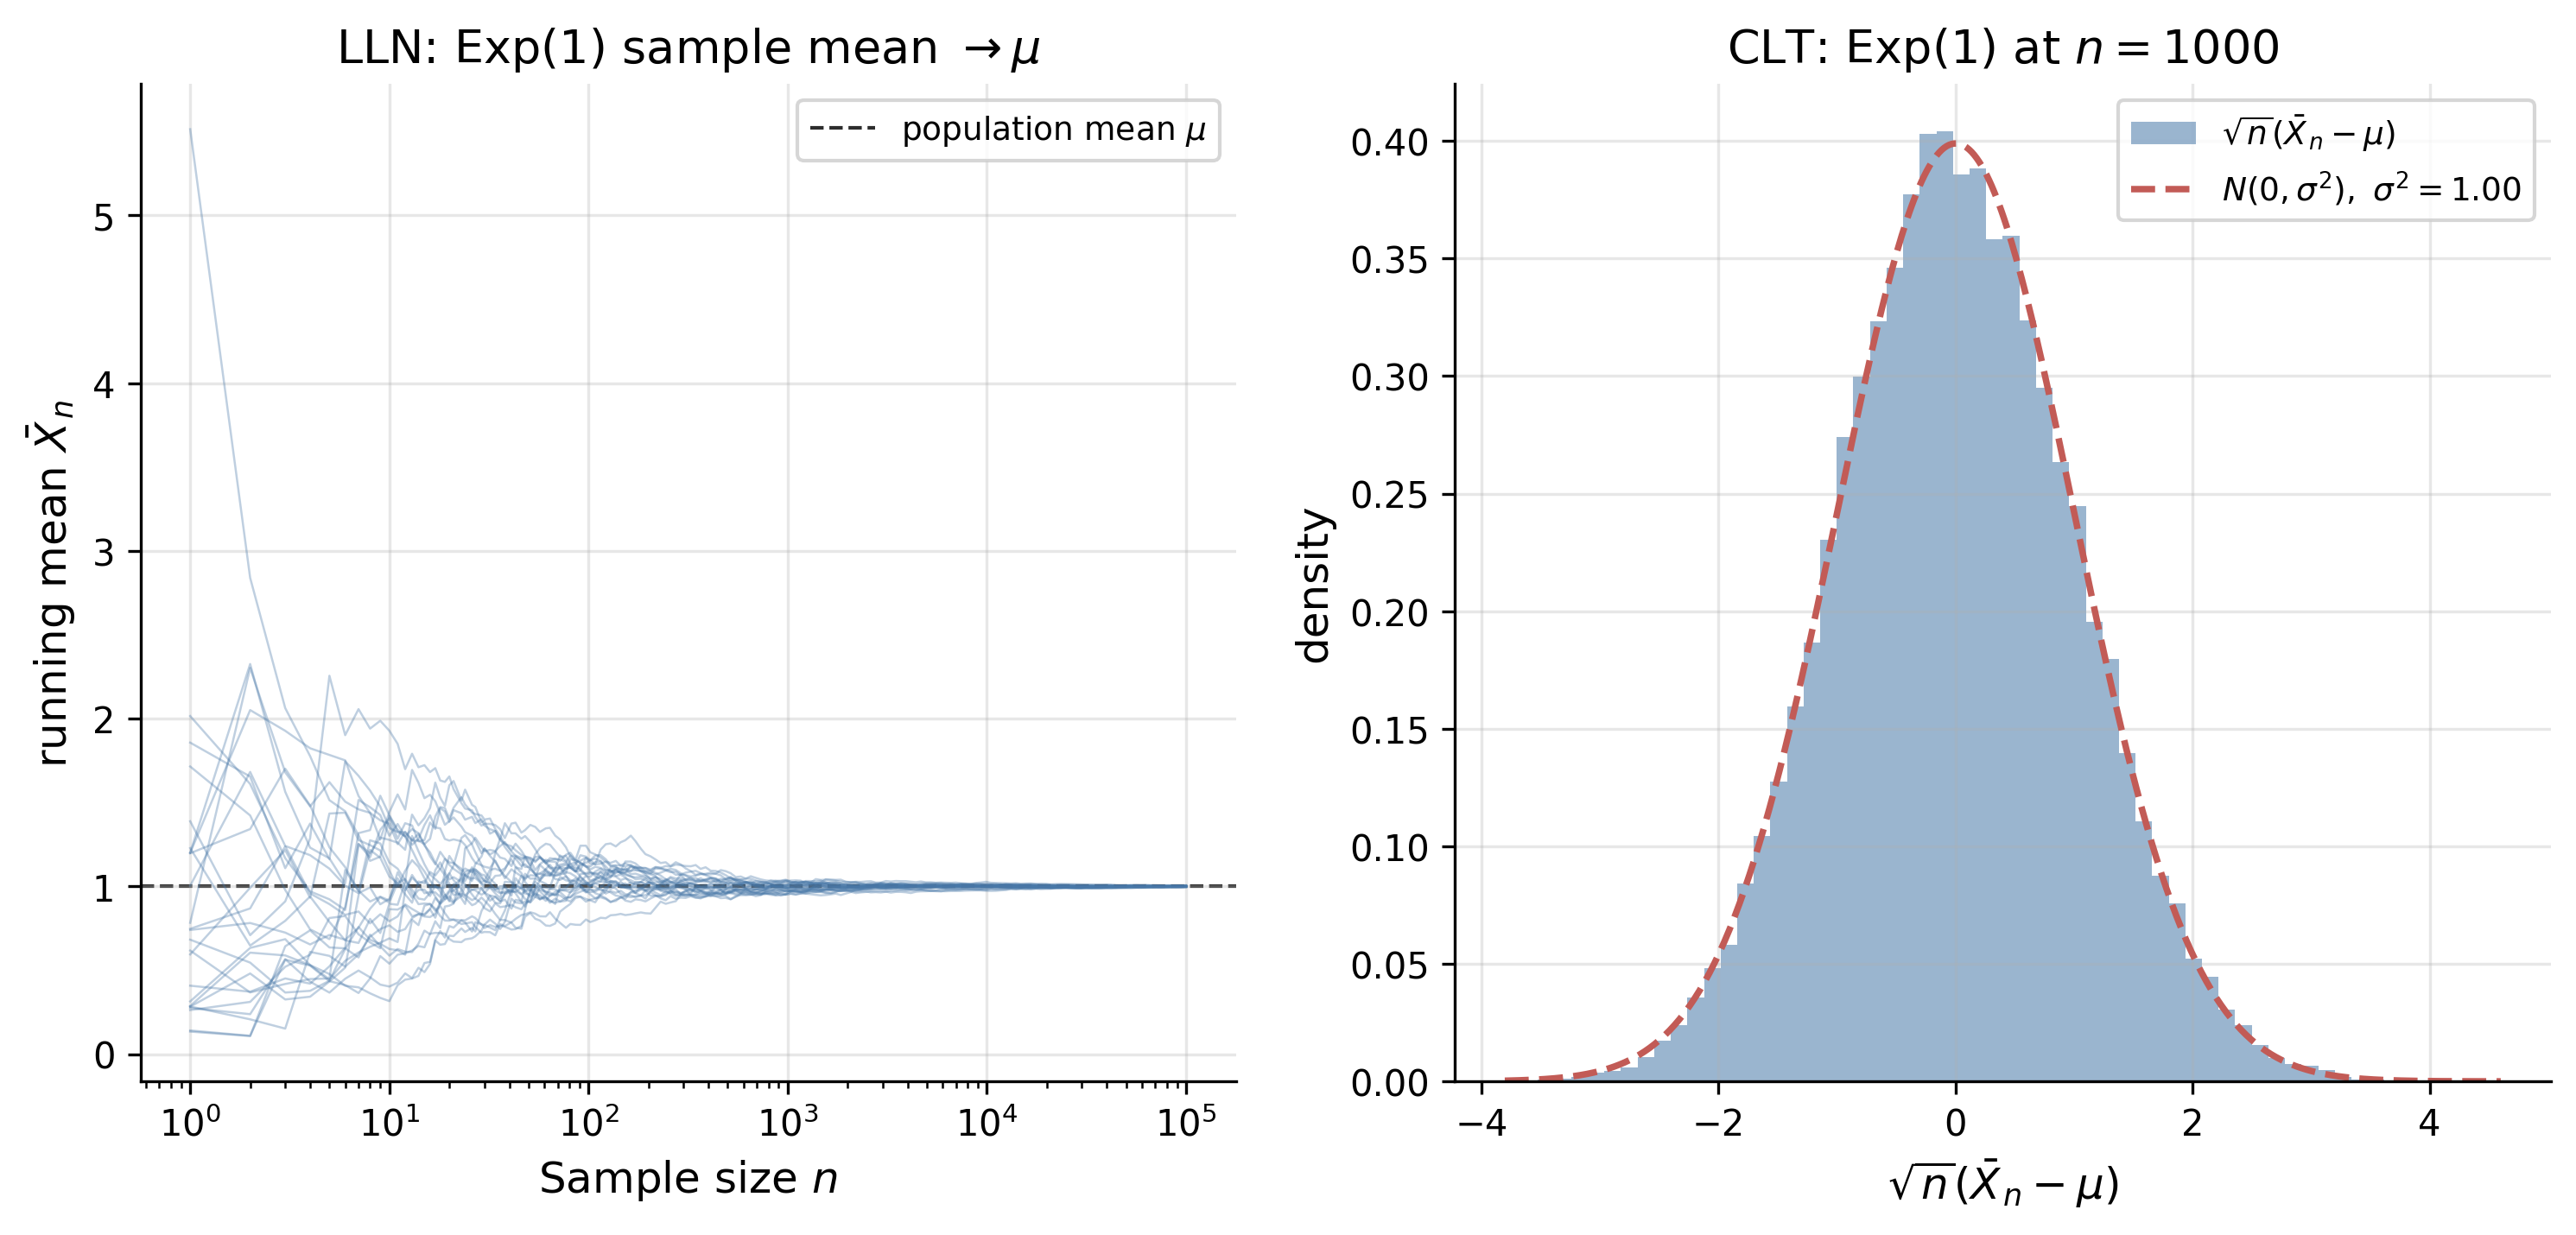
\includegraphics[width=0.95\textwidth]{../appA_preliminaries/sims/lln_clt.png}
\caption{Left: running sample mean $\bar X_n$ of $\mathrm{Exp}(1)$ draws against $n$ on a log scale, for 25 seeds, converging to the population mean $\mu = 1$ (dashed). Right: histogram of the rescaled fluctuation $\sqrt{n}(\bar X_n - \mu)$ for $\mathrm{Exp}(1)$ at $n = 1000$ over $40{,}000$ replicates, with the $N(0,\sigma^2)$ density overlaid (dashed).}
\label{fig:prelim_lln_clt}
\end{figure}

\begin{table}[h]
\centering
\caption{Central limit theorem for the rescaled sample mean $\sqrt{n}(\bar X_n - \mu)$ at $n=1000$, over 40{,}000 replicates, for three non-normal base distributions. The empirical variance matches $\sigma^2$ (ratio near one), and the skewness and excess kurtosis are near the normal values of zero, so the rescaled mean is approximately $N(0,\sigma^2)$ despite the skewed or discrete source. $D_{\mathrm{KS}}$ is the Kolmogorov-Smirnov distance to $N(0,\sigma^2)$.}
\label{tab:prelim_lln_clt}
\begin{tabular}{lccccc}
\hline
Distribution & $\sigma^2$ & Emp.\ var / $\sigma^2$ & Skew & Excess kurt.\ & $D_{\mathrm{KS}}$ \\
\hline
Exp$(1)$ & 1.0000 & 0.9972 & +0.0589 & -0.0176 & 0.0046 \\
Unif$(0,1)$ & 0.0833 & 1.0085 & +0.0108 & -0.0299 & 0.0047 \\
Bern$(0.3)$ & 0.2100 & 0.9970 & +0.0235 & -0.0510 & 0.0223 \\
\hline
\end{tabular}
\end{table}


\subsubsection{Martingale Convergence}

\begin{theorem}[Martingale convergence, \citet{williamsprob1991}; \citet{robbinssiegmund1971}]
\label{thm:prelim_martingale}
Let $(M_n)$ be a supermartingale adapted to a filtration $(\mathcal{F}_n)$, meaning $\mathbb{E}[M_{n+1} \mid \mathcal{F}_n] \leq M_n$, and suppose it is bounded in $L^1$, $\sup_n \mathbb{E}|M_n| < \infty$.\footnote{A \emph{filtration} $(\mathcal{F}_n)$ is the growing record of information through time. A process is a \emph{martingale} if $\mathbb{E}[M_{n+1} \mid \mathcal{F}_n] = M_n$, a \emph{supermartingale} if the conditional mean can only fall, $\mathbb{E}[M_{n+1} \mid \mathcal{F}_n] \leq M_n$. A martingale bounded in $[a,b]$ is automatically $L^1$-bounded.} Then $M_n$ converges almost surely to a finite limit $M_\infty$. Moreover, if $(Z_n)$ is a nonnegative adapted process with
\begin{equation}
\mathbb{E}[Z_{n+1} \mid \mathcal{F}_n] \leq (1 + a_n) Z_n - b_n + c_n,
\label{eq:prelim_robbins_siegmund}
\end{equation}
where $a_n, b_n, c_n \geq 0$ are $\mathcal{F}_n$-measurable with $\sum_n a_n < \infty$ and $\sum_n c_n < \infty$ almost surely, then $Z_n$ converges almost surely to a finite limit and $\sum_n b_n < \infty$ almost surely.
\end{theorem}

\begin{proof}
The plan is to bound how often the process can cross a fixed band, since a finite number of crossings rules out oscillation and forces convergence, and then to reduce the almost-supermartingale~\eqref{eq:prelim_robbins_siegmund} to that case. Fix a band $a < b$ and let $U_n[a,b]$ count the upcrossings of it by time $n$. Doob's upcrossing inequality bounds the expected count,\footnote{An \emph{upcrossing} is a passage of the process from below $a$ to above $b$. The inequality is proved by a betting strategy that buys when the process drops below $a$ and sells when it rises above $b$; each completed upcrossing books a profit of at least $b - a$, and the supermartingale property caps the expected profit, so the expected number of upcrossings is capped in turn.}
\begin{align*}
(b - a)\, \mathbb{E}\bigl[U_n[a,b]\bigr]
  &\leq \mathbb{E}\bigl[(M_n - a)^-\bigr] \leq |a| + \sup_n \mathbb{E}|M_n| && \text{(upcrossing inequality).}
\end{align*}
The right side is finite and does not grow with $n$, so the total number of upcrossings $U[a,b] = \lim_n U_n[a,b]$ is finite almost surely, and this holds simultaneously for every band with rational endpoints. A real sequence that upcrosses every rational band only finitely often cannot oscillate, so $M_n$ converges almost surely to some limit $M_\infty \in [-\infty, +\infty]$. Fatou's lemma with the $L^1$ bound gives $\mathbb{E}|M_\infty| \leq \liminf_n \mathbb{E}|M_n| < \infty$, so the limit is finite almost surely. For the almost-supermartingale, divide out the multiplicative drift and add the additive tail. The process $Z_n' = Z_n / \prod_{k<n}(1 + a_k) + \sum_{k \geq n} \tilde c_k$, with $\tilde c_k$ the discounted $c_k$, is a nonnegative supermartingale, so the first part applies and $Z_n'$ converges.\footnote{Adding the future $c$-tail is what cancels the upward push $c_n$ each step, leaving only the downward decrement $-\tilde b_n$; subtracting it would double the push.} Unwinding the two summable corrections returns the convergence of $Z_n$ and, from the accumulated decrements, $\sum_n b_n < \infty$ almost surely.\footnote{The bookkeeping is carried out in full by \citet{robbinssiegmund1971}. The two summability conditions on $a_n$ and $c_n$ are exactly what keep the discounting and the tail correction finite.}
\end{proof}

Martingale convergence is what turns a single noisy run into a convergence proof.\footnote{The almost-supermartingale form~\eqref{eq:prelim_robbins_siegmund} is the engine of the Robbins-Monro proof (Theorem~\ref{thm:prelim_robbins_monro}), and through it of the almost-sure convergence of Q-learning and $\mathrm{TD}(\lambda)$ in Section~\ref{sec:planning_learning} and the Nash-Q backup of Section~\ref{section:rl_games}.} A learning algorithm sees one trajectory, not an ensemble, so the guarantee it needs is almost-sure convergence of that path. Doob's theorem delivers exactly this once the running estimate is a bounded martingale or supermartingale, and the Robbins-Siegmund extension covers the case where the update contracts only up to summable perturbations, which is the shape every stochastic-approximation error takes. Figure~\ref{fig:prelim_martingale} follows a bounded martingale, the fraction of red balls in a P\'olya urn, and Table~\ref{tab:prelim_martingale} confirms the martingale property, the settling of every path, and that the random limits follow the predicted law.

\begin{figure}[t]
\centering
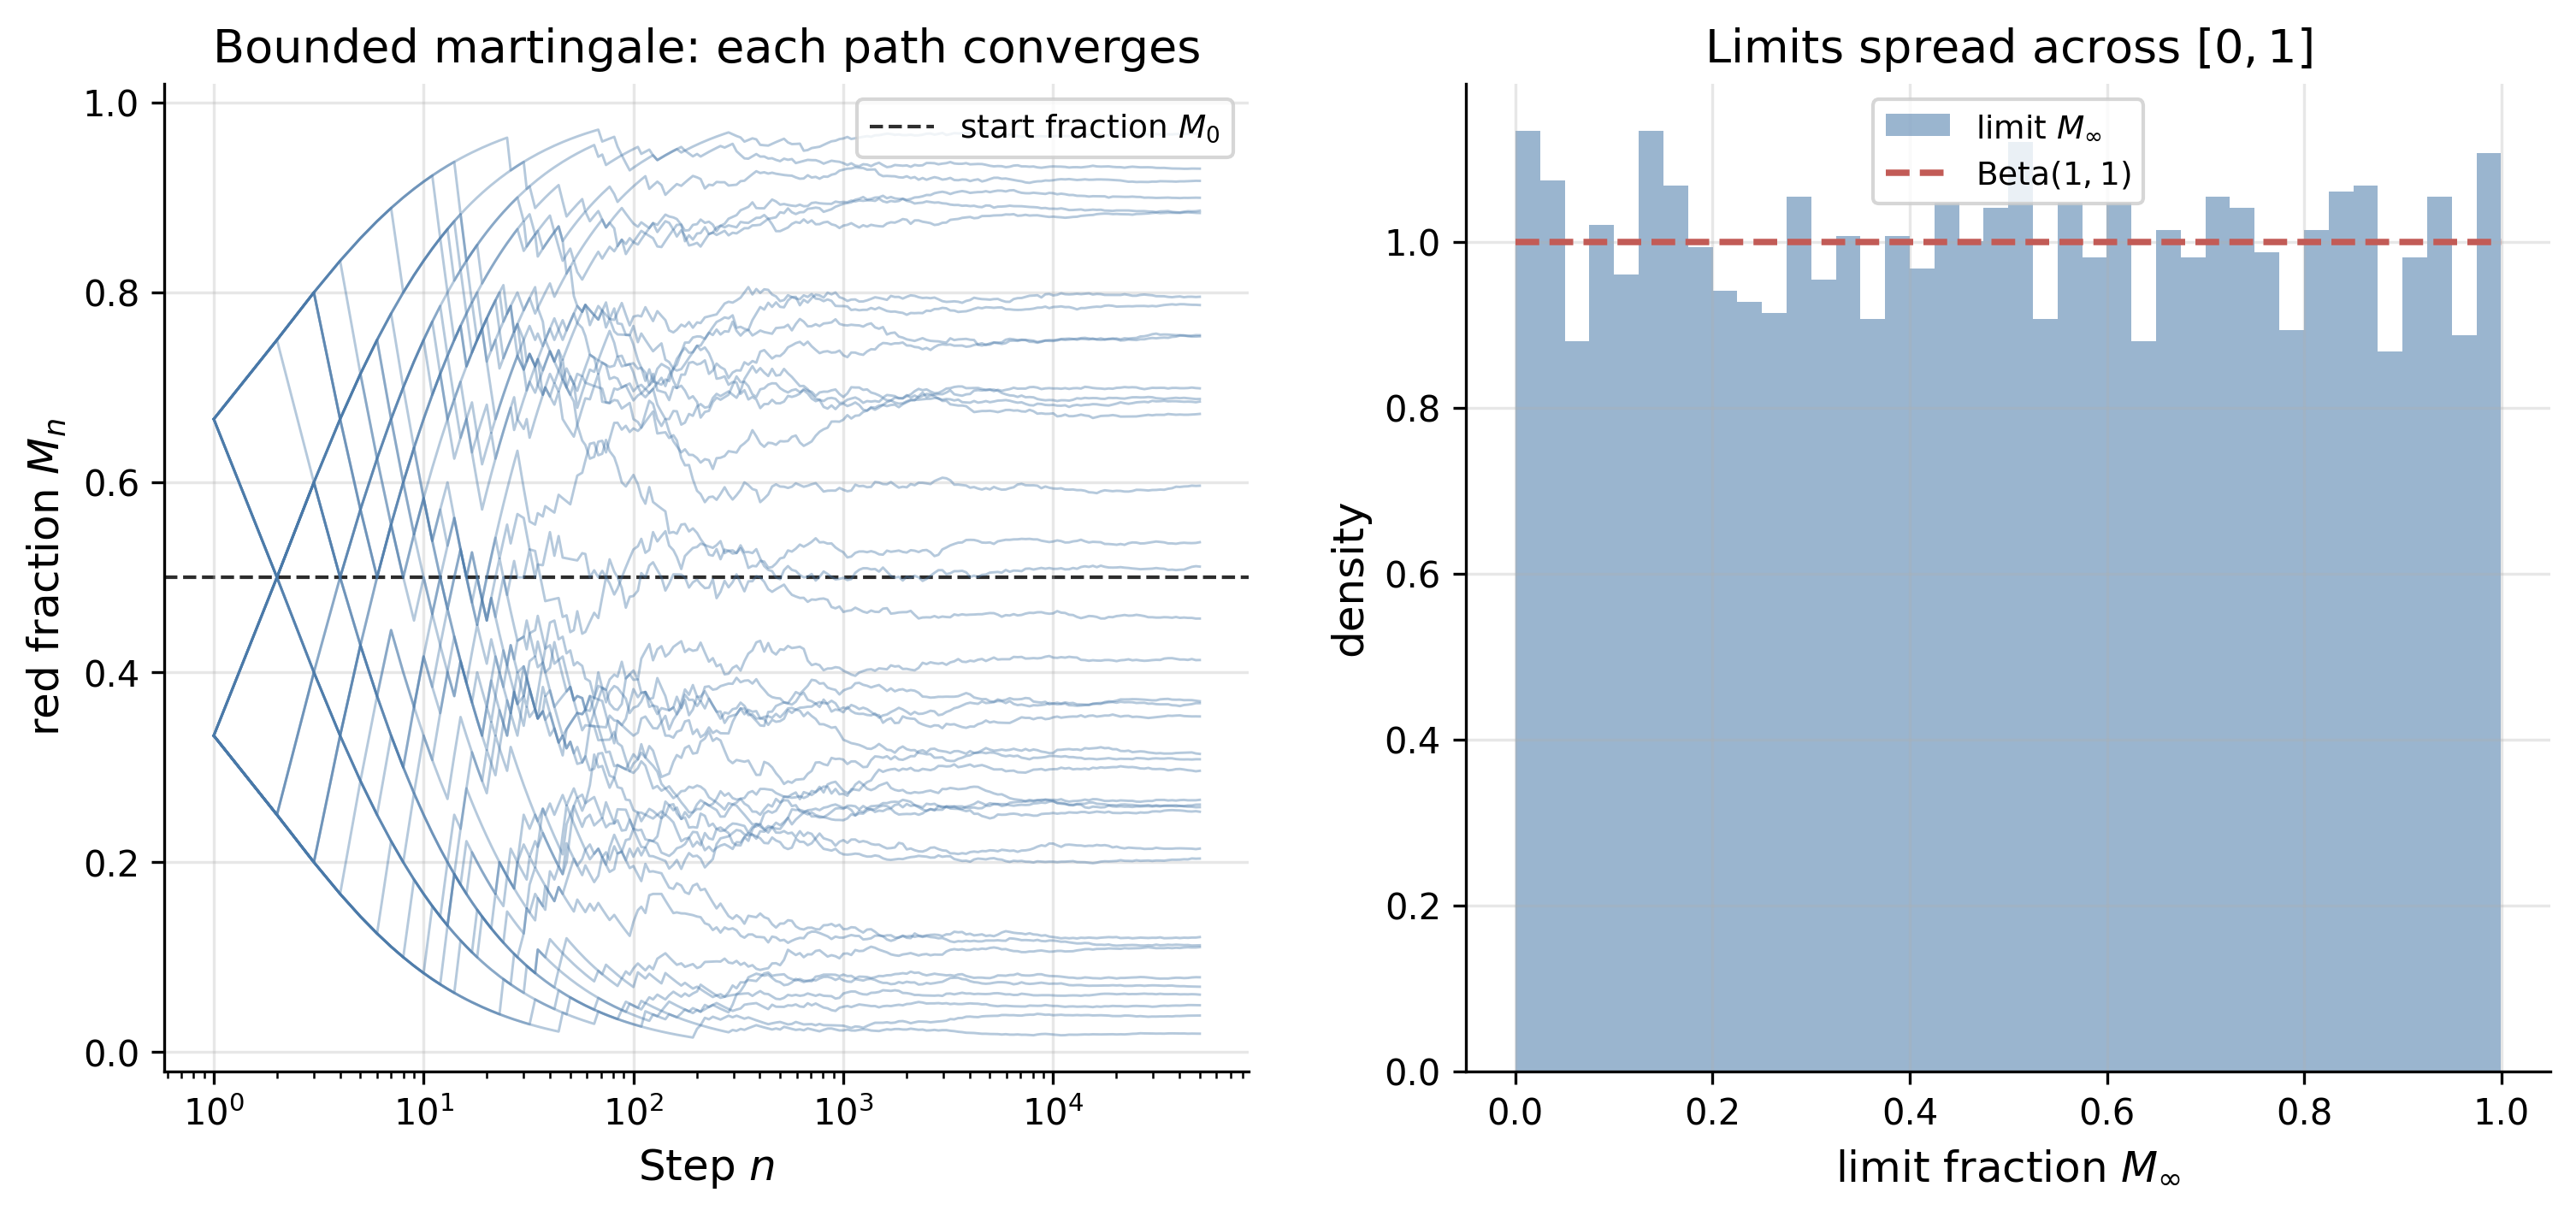
\includegraphics[width=0.95\textwidth]{../appA_preliminaries/sims/martingale_convergence.png}
\caption{Left: the red-ball fraction $M_n$ of a P\'olya urn from a $(1,1)$ start against the step $n$ on a log scale, for 40 seeds. Each bounded path converges to its own random limit. Right: the histogram of the limiting fractions across the ensemble, with the Beta$(1,1)$ density (dashed), the uniform law the theory predicts for this start.}
\label{fig:prelim_martingale}
\end{figure}

\begin{table}[h]
\centering
\caption{Almost-sure convergence of the P\'olya-urn martingale $M_n = (\text{red})/(\text{total})$ from a $(1,1)$ start. The one-step increment has mean zero, consistent with the martingale property (the theorem's conditional statement is proved analytically), every path settles (tail oscillation below 0.02 for the reported fraction of paths), and the random limits match the Beta$(1,1)$ law in mean, variance, and distribution ($D_{\mathrm{KS}}$). Limit ensemble of 6{,}000 urns.}
\label{tab:prelim_martingale}
\begin{tabular}{lcc}
\hline
Quantity & Simulated & Theory \\
\hline
Increment $E[M_{n+1}-M_n]$ & $-3.80e-07$ $\pm$ 9.3e-07 & $0$ \\
Paths settled (tail $< 0.02$) & 1.000 & $1$ \\
Limit mean & 0.4985 & 0.5000 \\
Limit variance & 0.0839 & 0.0833 \\
$D_{\mathrm{KS}}$ to Beta$(1,1)$ & 0.0072 & $0$ \\
\hline
\end{tabular}
\end{table}


\subsection{Calculus and Convex Analysis}
\label{prelim:convex}

Policy optimization, reward-model fitting, and constrained control all reduce to minimizing a function, usually by following its gradient. Four facts from convex analysis govern when that works and how fast. The first sets the convergence rate of gradient descent. The second turns a constrained problem into an unconstrained saddle point. The third differentiates an optimized value through its optimizer. The fourth is the continuity condition that ties this section back to the contraction arguments.

\subsubsection{Convexity and Gradient Descent}

\begin{theorem}[Gradient descent convergence, \citet{nesterov2018}]
\label{thm:prelim_gd}
Let $f$ be convex and $L$-smooth, and let $x^\star$ minimize $f$.\footnote{A differentiable $f$ is \emph{$L$-smooth} if its gradient is $L$-Lipschitz, $\|\nabla f(x) - \nabla f(y)\| \leq L\|x - y\|$, which bounds how fast the slope can change. It is \emph{$\mu$-strongly convex} if $f(x) - \tfrac{\mu}{2}\|x\|^2$ is still convex, so $f$ curves up at least as fast as a quadratic of curvature $\mu$.} Gradient descent with step $1/L$, $x_{k+1} = x_k - \tfrac{1}{L}\nabla f(x_k)$, satisfies
\begin{equation}
f(x_k) - f(x^\star) \leq \frac{L\,\|x_0 - x^\star\|^2}{2k}.
\label{eq:prelim_gd_sublinear}
\end{equation}
If in addition $f$ is $\mu$-strongly convex, with condition number $\kappa = L/\mu$, the iterates converge geometrically,
\begin{equation}
\|x_k - x^\star\| \leq \Bigl(1 - \tfrac{\mu}{L}\Bigr)^{k} \|x_0 - x^\star\|.
\label{eq:prelim_gd_linear}
\end{equation}
\end{theorem}

\begin{proof}
The plan is to turn smoothness into a guaranteed per-step decrease, convert that decrease into the $O(1/k)$ rate with convexity, and sharpen it to a geometric rate when strong convexity is available. Smoothness gives the descent lemma, a quadratic upper model of $f$,
\begin{align*}
f(y) &\leq f(x) + \langle \nabla f(x), y - x \rangle + \tfrac{L}{2}\|y - x\|^2 && \text{($L$-smoothness).}
\end{align*}
Evaluating at the gradient step $y = x - \tfrac{1}{L}\nabla f(x)$ collapses the right side to
\begin{align*}
f(x_{k+1}) &\leq f(x_k) - \tfrac{1}{2L}\|\nabla f(x_k)\|^2 && \text{(insert the step),}
\end{align*}
so each step strictly decreases $f$ unless the gradient is zero. Convexity bounds the optimality gap by the gradient, $f(x_k) - f(x^\star) \leq \langle \nabla f(x_k), x_k - x^\star \rangle$, and combined with the decrease the squared distance $\|x_k - x^\star\|^2$ is nonincreasing; summing the per-step decreases telescopes to~\eqref{eq:prelim_gd_sublinear}.\footnote{The telescoping uses $\|x_{k+1} - x^\star\|^2 = \|x_k - x^\star\|^2 - \tfrac{2}{L}\langle \nabla f(x_k), x_k - x^\star\rangle + \tfrac{1}{L^2}\|\nabla f(x_k)\|^2$ and the two displayed inequalities; the full algebra is in \citet{nesterov2018}.} When $f$ is $\mu$-strongly convex the gradient step $T(x) = x - \tfrac{1}{L}\nabla f(x)$ is a contraction. Its fixed point is $x^\star$, since $\nabla f(x^\star) = 0$, and strong convexity with smoothness makes it a $(1 - \mu/L)$-contraction,\footnote{Write $\nabla f(x) - \nabla f(y) = \bar H (x - y)$ with the averaged Hessian $\bar H = \int_0^1 \nabla^2 f\bigl(y + s(x-y)\bigr)\,ds$, which satisfies $\mu I \preceq \bar H \preceq L I$. Then $T(x) - T(y) = (I - \bar H/L)(x - y)$ and $\|I - \bar H/L\| = \max_{\lambda \in [\mu, L]} |1 - \lambda/L| = 1 - \mu/L$, so $\|T(x) - T(y)\| \leq (1 - \mu/L)\|x - y\|$. The gradient step is thus a contraction, and gradient descent is the contraction-mapping principle of Section~\ref{prelim:fixedpoints} applied to $T$, with the minimizer as the fixed point.} so
\begin{align*}
\|x_{k+1} - x^\star\| = \|T(x_k) - T(x^\star)\| &\leq \bigl(1 - \tfrac{\mu}{L}\bigr)\|x_k - x^\star\| && \text{(contraction),}
\end{align*}
and iterating gives~\eqref{eq:prelim_gd_linear}.
\end{proof}

The split between the two rates is the split between hard and easy problems.\footnote{Gradient methods are the workhorse of policy optimization, the policy-gradient ascent of Section~\ref{sec:policy_gradient} and the actor-critic updates of Section~\ref{sec:actor_critic}, and of the reward-model and policy fitting in the alignment objective of Section~\ref{sec:lcpo}. The condition number $\kappa = L/\mu$ is what separates a fast-training objective from a slow one.} On a general smooth convex objective gradient descent closes the gap at the sublinear rate $O(1/k)$. Strong convexity, the curvature that keeps the objective from flattening near the optimum, upgrades this to the geometric rate $(1 - \mu/L)^k$, so the iteration count to a fixed accuracy scales with the condition number $\kappa = L/\mu$. The linear rate is exactly the Banach contraction applied to the gradient map, and it holds for any strongly convex smooth objective, not only the quadratics used here to make the constant sharp. Figure~\ref{fig:prelim_gd} shows the geometric decay at three condition numbers and the general bound holding for the worst-conditioned case, and Table~\ref{tab:prelim_gd} confirms the measured per-step contraction equals $1 - \mu/L$.

\begin{figure}[t]
\centering
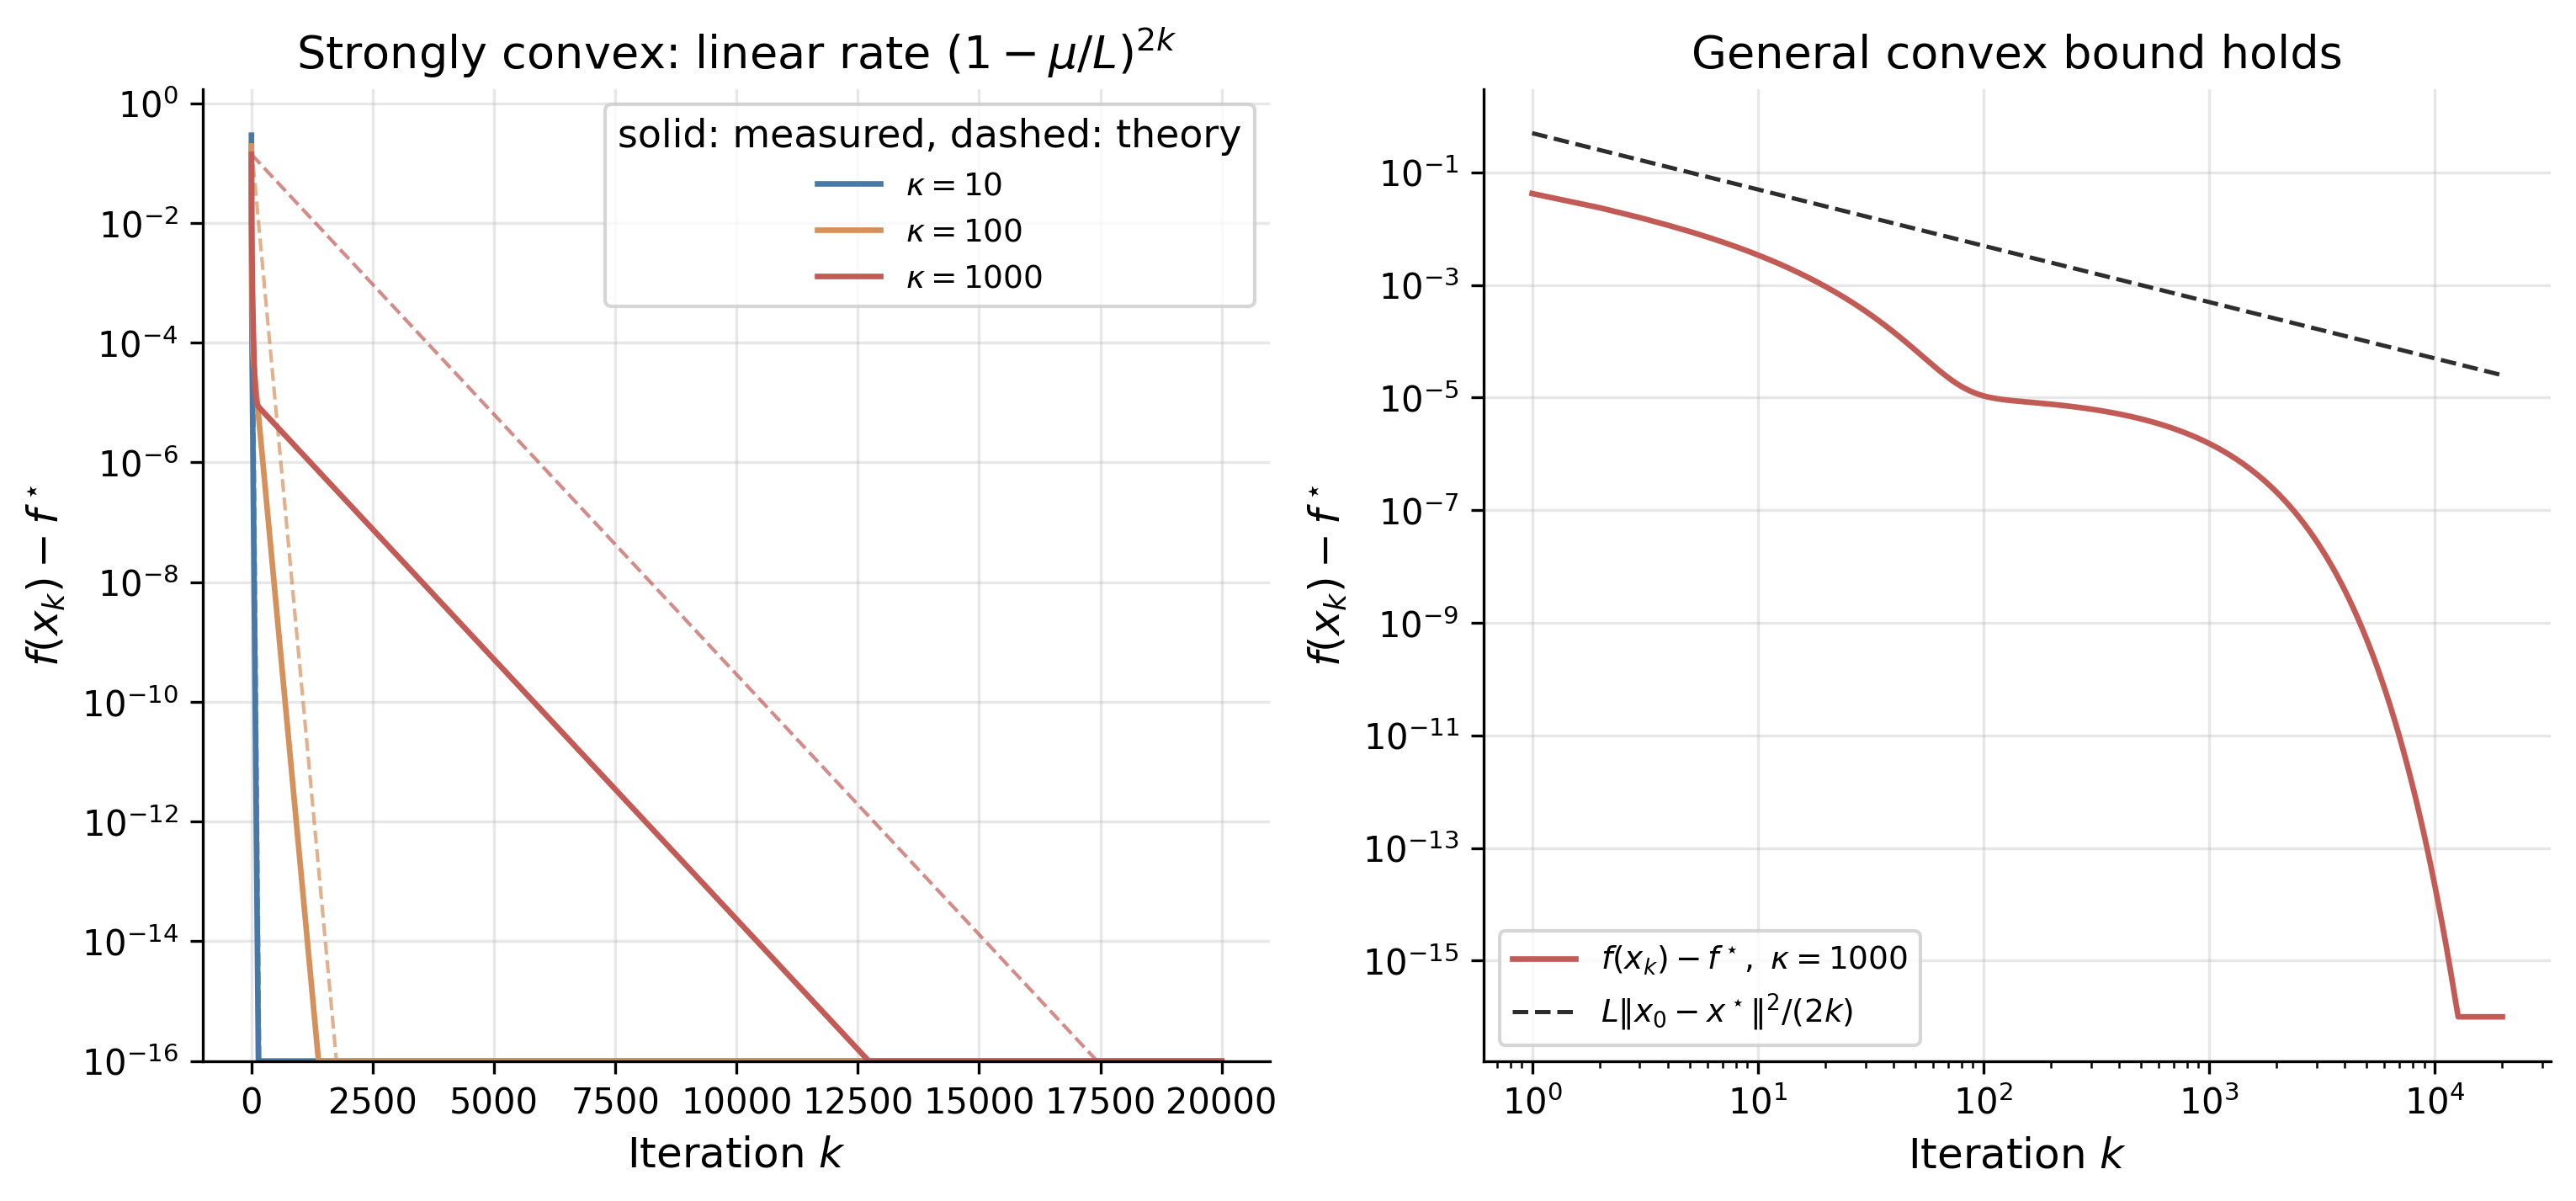
\includegraphics[width=0.95\textwidth]{../appA_preliminaries/sims/gradient_descent.png}
\caption{Left: optimality gap $f(x_k) - f^\star$ of gradient descent with step $1/L$ on strongly convex quadratics at condition numbers $\kappa \in \{10, 100, 1000\}$ (solid), against the geometric envelope $(1 - \mu/L)^{2k}$ (dashed), on a log scale. Right: the worst-conditioned case ($\kappa = 1000$) against the general convex bound $L\|x_0 - x^\star\|^2/(2k)$ (dashed), on log-log axes, which it stays below throughout.}
\label{fig:prelim_gd}
\end{figure}

\begin{table}[h]
\centering
\caption{Gradient descent with step $1/L$ on strongly convex quadratics at three condition numbers $\kappa = L/\mu$. The asymptotic per-step contraction of the iterate error, read off the tail of the closed-form trajectory, equals the linear rate $1 - \mu/L$ by construction, so the iteration count to a fixed tolerance grows with $\kappa$. The general smooth-convex bound $f(x_k) - f^\star \leq L\|x_0 - x^\star\|^2/(2k)$ holds throughout (ratio $\leq 1$). Mean $\pm$ SE over 20 random initial points.}
\label{tab:prelim_gd}
\begin{tabular}{ccccc}
\hline
$\kappa$ & $\mu/L$ & Per-step factor & Theory $1-\mu/L$ & $O(1/k)$ bound ratio \\
\hline
10 & 0.1000 & 0.90000 $\pm$ 4e-08 & 0.90000 & 0.105 \\
100 & 0.0100 & 0.99000 $\pm$ 7e-17 & 0.99000 & 0.122 \\
1000 & 0.0010 & 0.99900 $\pm$ 2e-17 & 0.99900 & 0.120 \\
\hline
\end{tabular}
\end{table}


\subsubsection{Lagrangian Duality}

\begin{theorem}[Weak and strong duality, \citet{boydvandenberghe2004}; \citet{sion1958}]
\label{thm:prelim_duality}
Consider the program $p^\star = \min_x f(x)$ subject to $g_i(x) \leq 0$ for $i = 1, \ldots, m$, with Lagrangian $L(x, \lambda) = f(x) + \sum_i \lambda_i g_i(x)$ and dual function $q(\lambda) = \inf_x L(x, \lambda)$ for $\lambda \geq 0$.\footnote{The multipliers $\lambda_i \geq 0$ price the constraints. The \emph{dual function} $q(\lambda) = \inf_x L(x,\lambda)$ is the best lower bound the prices $\lambda$ can certify, and it is concave in $\lambda$ as an infimum of affine functions, whatever $f$ and $g_i$ are.} Let $d^\star = \sup_{\lambda \geq 0} q(\lambda)$. Then weak duality always holds,
\begin{equation}
d^\star \leq p^\star,
\label{eq:prelim_weak_duality}
\end{equation}
and if $f$ and the $g_i$ are convex and a strictly feasible point exists, so that $g_i(\bar x) < 0$ for some $\bar x$ and all $i$ (Slater's condition), then strong duality holds, $d^\star = p^\star$, attained at a saddle point $(x^\star, \lambda^\star)$,
\begin{equation}
L(x^\star, \lambda) \leq L(x^\star, \lambda^\star) \leq L(x, \lambda^\star) \quad \text{for all } x, \ \lambda \geq 0.
\label{eq:prelim_saddle}
\end{equation}
\end{theorem}

\begin{proof}
The plan is to get weak duality from the sign of the multipliers directly, and strong duality from the convexity of the value function, which under Slater admits a supporting hyperplane whose slope is the optimal multiplier. For weak duality take any feasible $x$ and any $\lambda \geq 0$,
\begin{align*}
q(\lambda) = \inf_{x'} L(x', \lambda) \leq L(x, \lambda) = f(x) + \sum_i \lambda_i g_i(x)
  &\leq f(x) && \text{($\lambda_i \geq 0$, $g_i(x) \leq 0$).}
\end{align*}
Taking the infimum over feasible $x$ gives $q(\lambda) \leq p^\star$, and the supremum over $\lambda \geq 0$ gives~\eqref{eq:prelim_weak_duality}, with no convexity used. For strong duality consider the value set $\mathcal{A} = \{(u, t) : g_i(x) \leq u_i,\ f(x) \leq t \text{ for some } x\}$, which is convex when $f$ and the $g_i$ are convex.\footnote{The point $(0, p^\star)$ lies on the boundary of $\mathcal{A}$. A supporting hyperplane there has a normal $(\lambda^\star, \mu)$, pointing into $\mathcal{A}$, with $\lambda^\star \geq 0$ and $\mu \geq 0$; Slater's strictly feasible point forces $\mu > 0$, so the hyperplane is nonvertical and can be normalized to $\mu = 1$. The full separation argument is in \citet{boydvandenberghe2004}.} The supporting hyperplane at $(0, p^\star)$ yields multipliers $\lambda^\star \geq 0$ with $q(\lambda^\star) = p^\star$, so $d^\star = p^\star$. The optimal pair then satisfies~\eqref{eq:prelim_saddle}, equivalently the minimax identity $\min_x \max_{\lambda \geq 0} L(x, \lambda) = \max_{\lambda \geq 0} \min_x L(x, \lambda)$. Strong duality establishes this identity here; for a convex-concave payoff it holds generally once one of the two domains is compact, which is the minimax theorem of \citet{sion1958}.
\end{proof}

Duality is how a constrained problem becomes an unconstrained one.\footnote{Lagrangian duality turns the constrained and robust value problems of Section~\ref{section:dist_robust_constrained} into unconstrained saddle points solved by primal-dual iteration, and it is the mechanism behind the KL-regularized alignment objective of Section~\ref{sec:lcpo}, where the constraint multiplier trades reward against divergence from the reference policy.} Rather than optimize subject to constraints, one forms the Lagrangian and searches for its saddle point, ascending in the multipliers and descending in the variables. Weak duality guarantees every setting of the multipliers certifies a lower bound on the optimum, and strong duality, which the convex constrained problems in reinforcement learning enjoy under a feasibility condition, guarantees the bound is tight. Figure~\ref{fig:prelim_duality} solves a convex quadratic program through its dual, and Table~\ref{tab:prelim_duality} confirms the dual value stays below the primal optimum throughout and closes to it, with complementary slackness holding at the solution.

\begin{figure}[t]
\centering
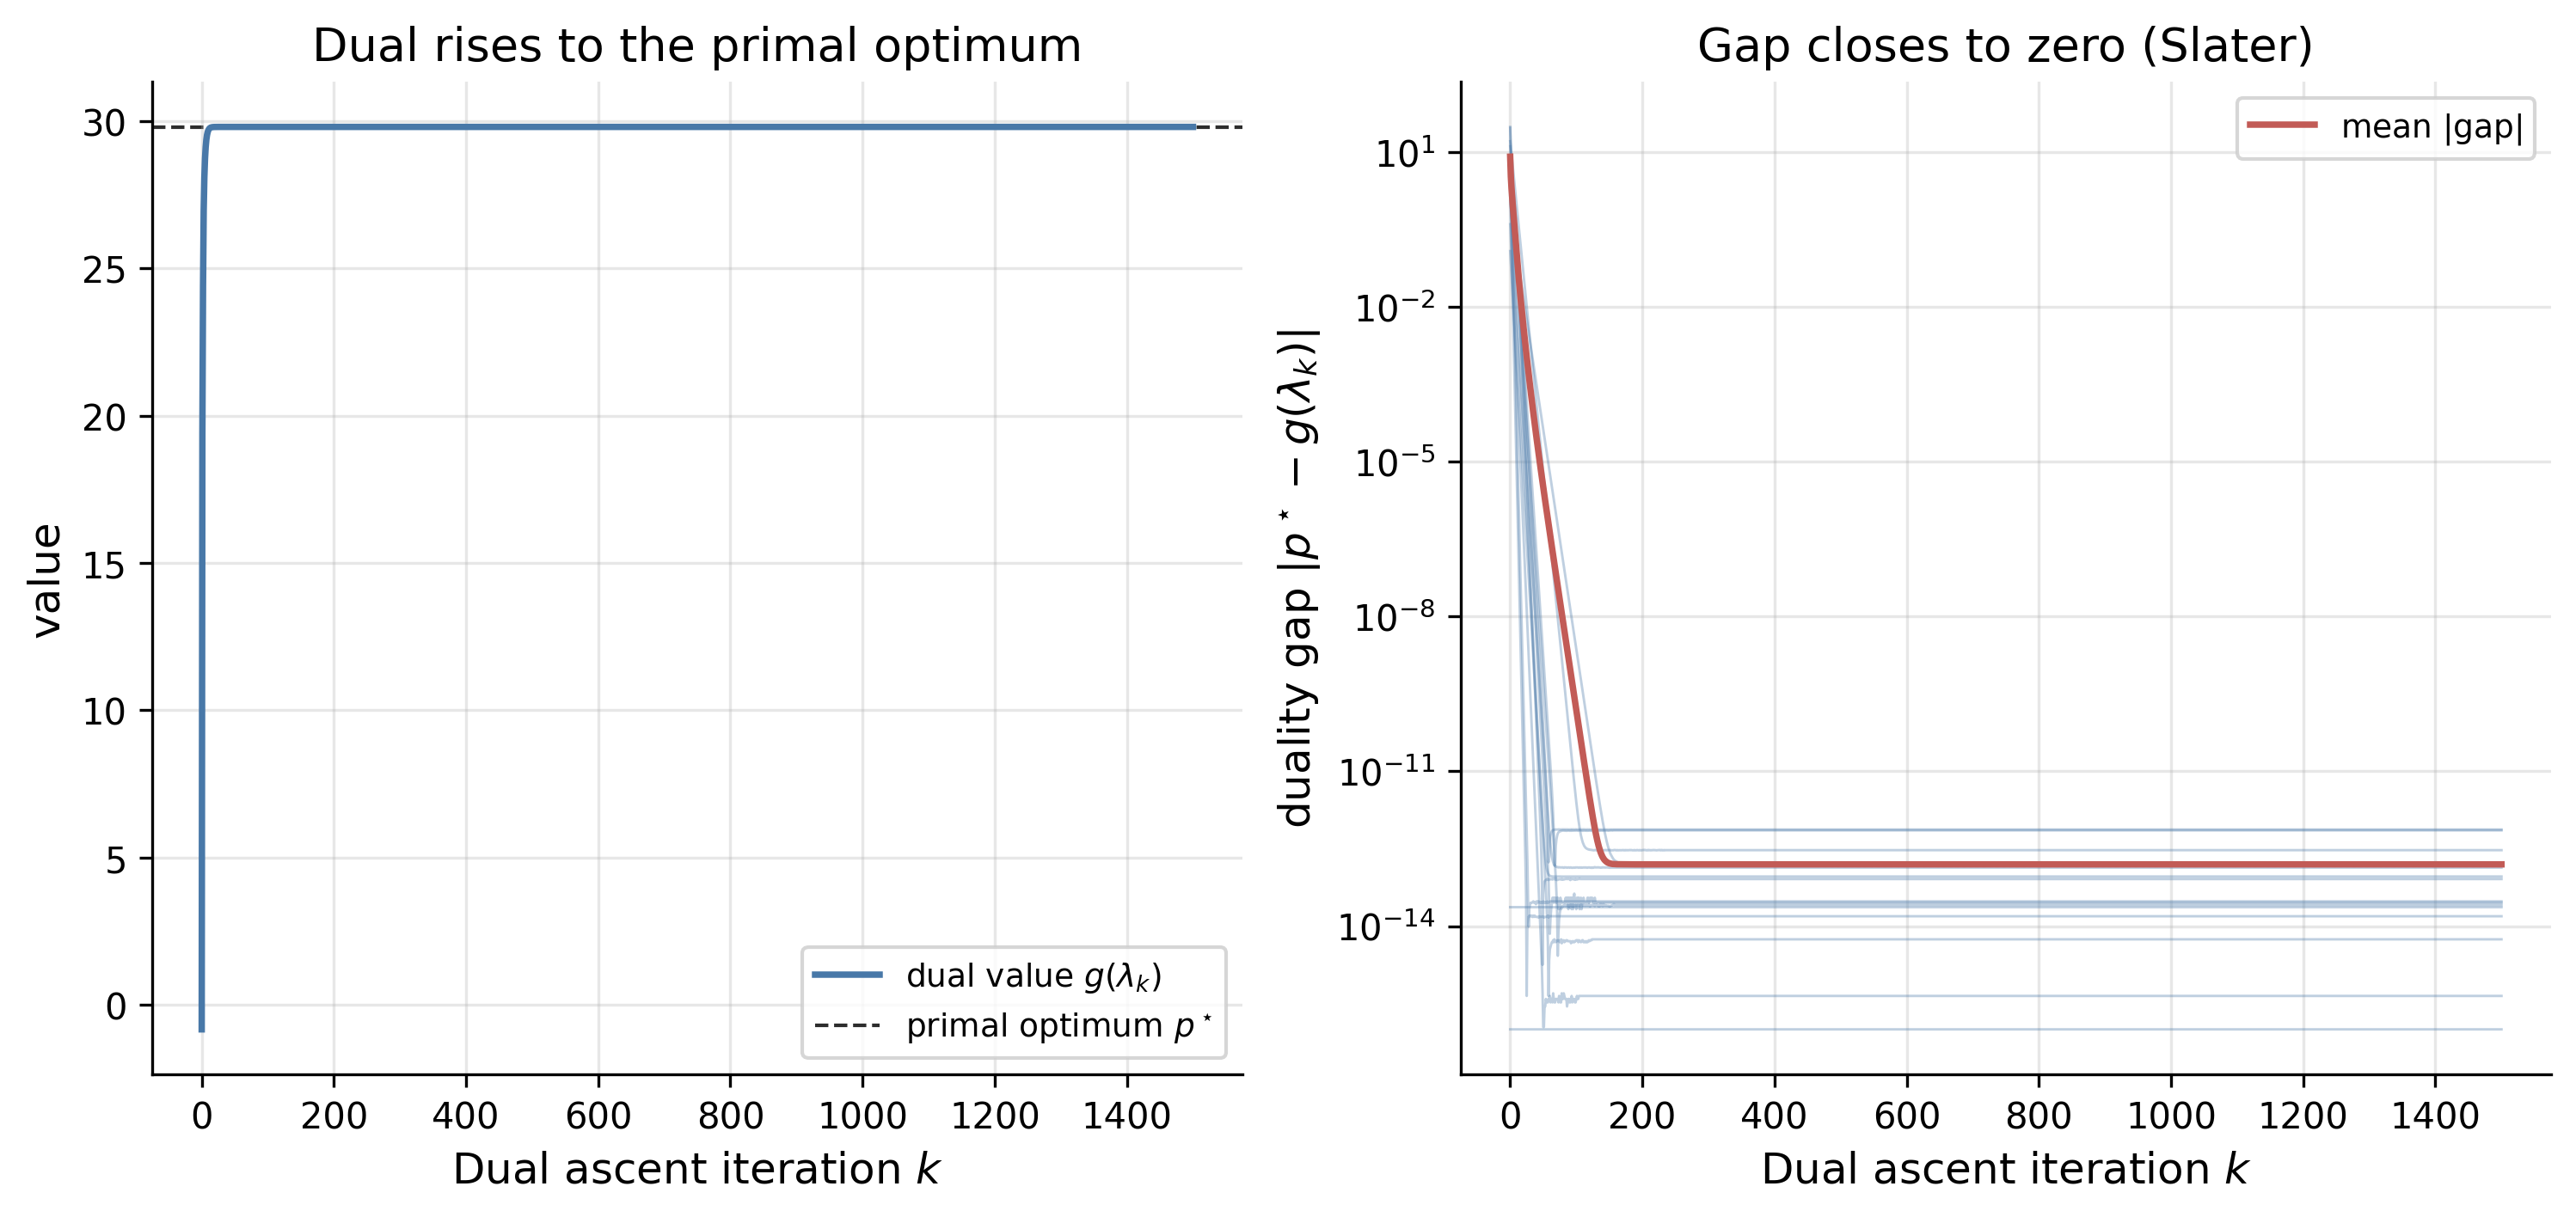
\includegraphics[width=0.95\textwidth]{../appA_preliminaries/sims/lagrangian_duality.png}
\caption{Left: dual value $g(\lambda_k)$ of a convex quadratic program under projected dual ascent, rising to the primal optimum $p^\star$ (dashed) from below. Right: the duality gap $|p^\star - g(\lambda_k)|$ against the iteration, for 15 random instances (thin) and their mean (thick), on a log scale, closing to solver precision because a strictly feasible point exists.}
\label{fig:prelim_duality}
\end{figure}

\begin{table}[h]
\centering
\caption{Lagrangian duality for a convex quadratic program $\min \tfrac12 x^\top Q x + c^\top x$ s.t.\ $Ax \leq b$, solved through its dual by projected gradient ascent, over 15 random instances. The dual value is a lower bound on the primal optimum $p^\star$ at every iteration (weak duality holds on all iterates), and the duality gap closes to zero because a strictly feasible point exists (Slater's condition, strong duality). The complementary-slackness residual $\max_i |\lambda_i (Ax - b)_i|$ vanishes at the solution. $p^\star$ is computed independently by SLSQP.}
\label{tab:prelim_duality}
\begin{tabular}{lc}
\hline
Quantity & Value \\
\hline
Final duality gap $|p^\star - g(\lambda)|$ & $\leq 7.4e-13$ (solver precision) \\
Weak duality holds (fraction of seeds) & 1.000 \\
Complementary slackness $\max_i|\lambda_i(Ax-b)_i|$ & $3.4e-15$ (max $1.9e-14$) \\
Active constraints (mean) & 1.5 of 5 \\
\hline
\end{tabular}
\end{table}


\subsubsection{The Envelope Theorem}

\begin{theorem}[Envelope theorem, \citet{milgromsegal2002}; \citet{danskin1967}]
\label{thm:prelim_envelope}
Let $V(\theta) = \max_{a \in A} f(a, \theta)$ be a value function, with $A$ compact, $f$ and its partial $\partial_\theta f$ jointly continuous in $(a, \theta)$, and $a^\star(\theta) \in \arg\max_a f(a, \theta)$ a maximizer.\footnote{The \emph{value function} $V$ records the best attainable payoff as the parameter $\theta$ moves. It is convex in $\theta$ when $f$ is convex in $\theta$, being a maximum of such functions, but it need not be smooth. Compactness of $A$ with continuity of $f$ makes the maximum attained.} If the maximizer $a^\star(\theta)$ is unique, then $V$ is differentiable at $\theta$ and
\begin{equation}
V'(\theta) = \frac{\partial f}{\partial \theta}\bigl(a^\star(\theta), \theta\bigr).
\label{eq:prelim_envelope}
\end{equation}
The change in the maximizer contributes nothing to first order. When the maximizer is not unique, $V$ still has one-sided derivatives, given by the extreme values of $\partial_\theta f$ over the set of maximizers.\footnote{This is Danskin's directional-derivative statement: $V'(\theta; d) = \max_{a \in \arg\max} \partial_\theta f(a, \theta)\, d$. A unique maximizer collapses the interval of one-sided slopes to the single derivative~\eqref{eq:prelim_envelope}; multiple maximizers leave a kink.}
\end{theorem}

\begin{proof}
The plan is to trap the difference quotient of $V$ between two partial-derivative evaluations that pinch to the same limit at a unique maximizer. Fix $\theta$ and take $\theta' > \theta$. Because $a^\star(\theta)$ is feasible at $\theta'$ and $a^\star(\theta')$ is optimal there, while the reverse holds at $\theta$,
\begin{align*}
V(\theta') - V(\theta)
  &\geq f(a^\star(\theta), \theta') - f(a^\star(\theta), \theta) && \text{($a^\star(\theta)$ feasible at $\theta'$)} \\
V(\theta') - V(\theta)
  &\leq f(a^\star(\theta'), \theta') - f(a^\star(\theta'), \theta) && \text{($a^\star(\theta')$ feasible at $\theta$).}
\end{align*}
Dividing by $\theta' - \theta > 0$ and letting $\theta' \to \theta$, the lower bound tends to $\partial_\theta f(a^\star(\theta), \theta)$ by differentiability of $f$ in $\theta$, and the upper bound tends to the same limit because the argmax is upper hemicontinuous by Berge's maximum theorem, a unique maximizer upgrades this to $a^\star(\theta') \to a^\star(\theta)$, and $\partial_\theta f$ is jointly continuous. The two bounds squeeze the difference quotient, giving~\eqref{eq:prelim_envelope}. The same sandwich from the left matches the one-sided derivatives, and when the maximizer is not unique the two sides settle on the extreme maximizer slopes, which is Danskin's statement.
\end{proof}

The envelope theorem is why one can differentiate an optimized value without tracking the optimizer.\footnote{Danskin's form supplies the gradient of the inner maximization in the robust value operators of Section~\ref{section:dist_robust_constrained}, where the derivative of the worst-case value is the derivative at the worst-case model. The envelope identity underlies the policy-gradient theorem of Section~\ref{sec:policy_gradient} and the sensitivity of estimated value functions to structural parameters in Section~\ref{section:rl_econ_models}.} In dynamic programming the derivative of the value with respect to a state or a parameter equals the derivative of the one-step return at the optimal action, the Benveniste-Scheinkman identity, which is what makes marginal-value conditions tractable. In robust and minimax control, Danskin's form gives the gradient of a worst-case objective as the gradient evaluated at the worst case, so the inner maximization can be treated as fixed when differentiating. Figure~\ref{fig:prelim_envelope} shows the value as the upper envelope of a family of curves, tangent to each where that member is optimal, and Table~\ref{tab:prelim_envelope} confirms that differentiating a numerically maximized value reproduces the partial derivative at the maximizer.

\begin{figure}[t]
\centering
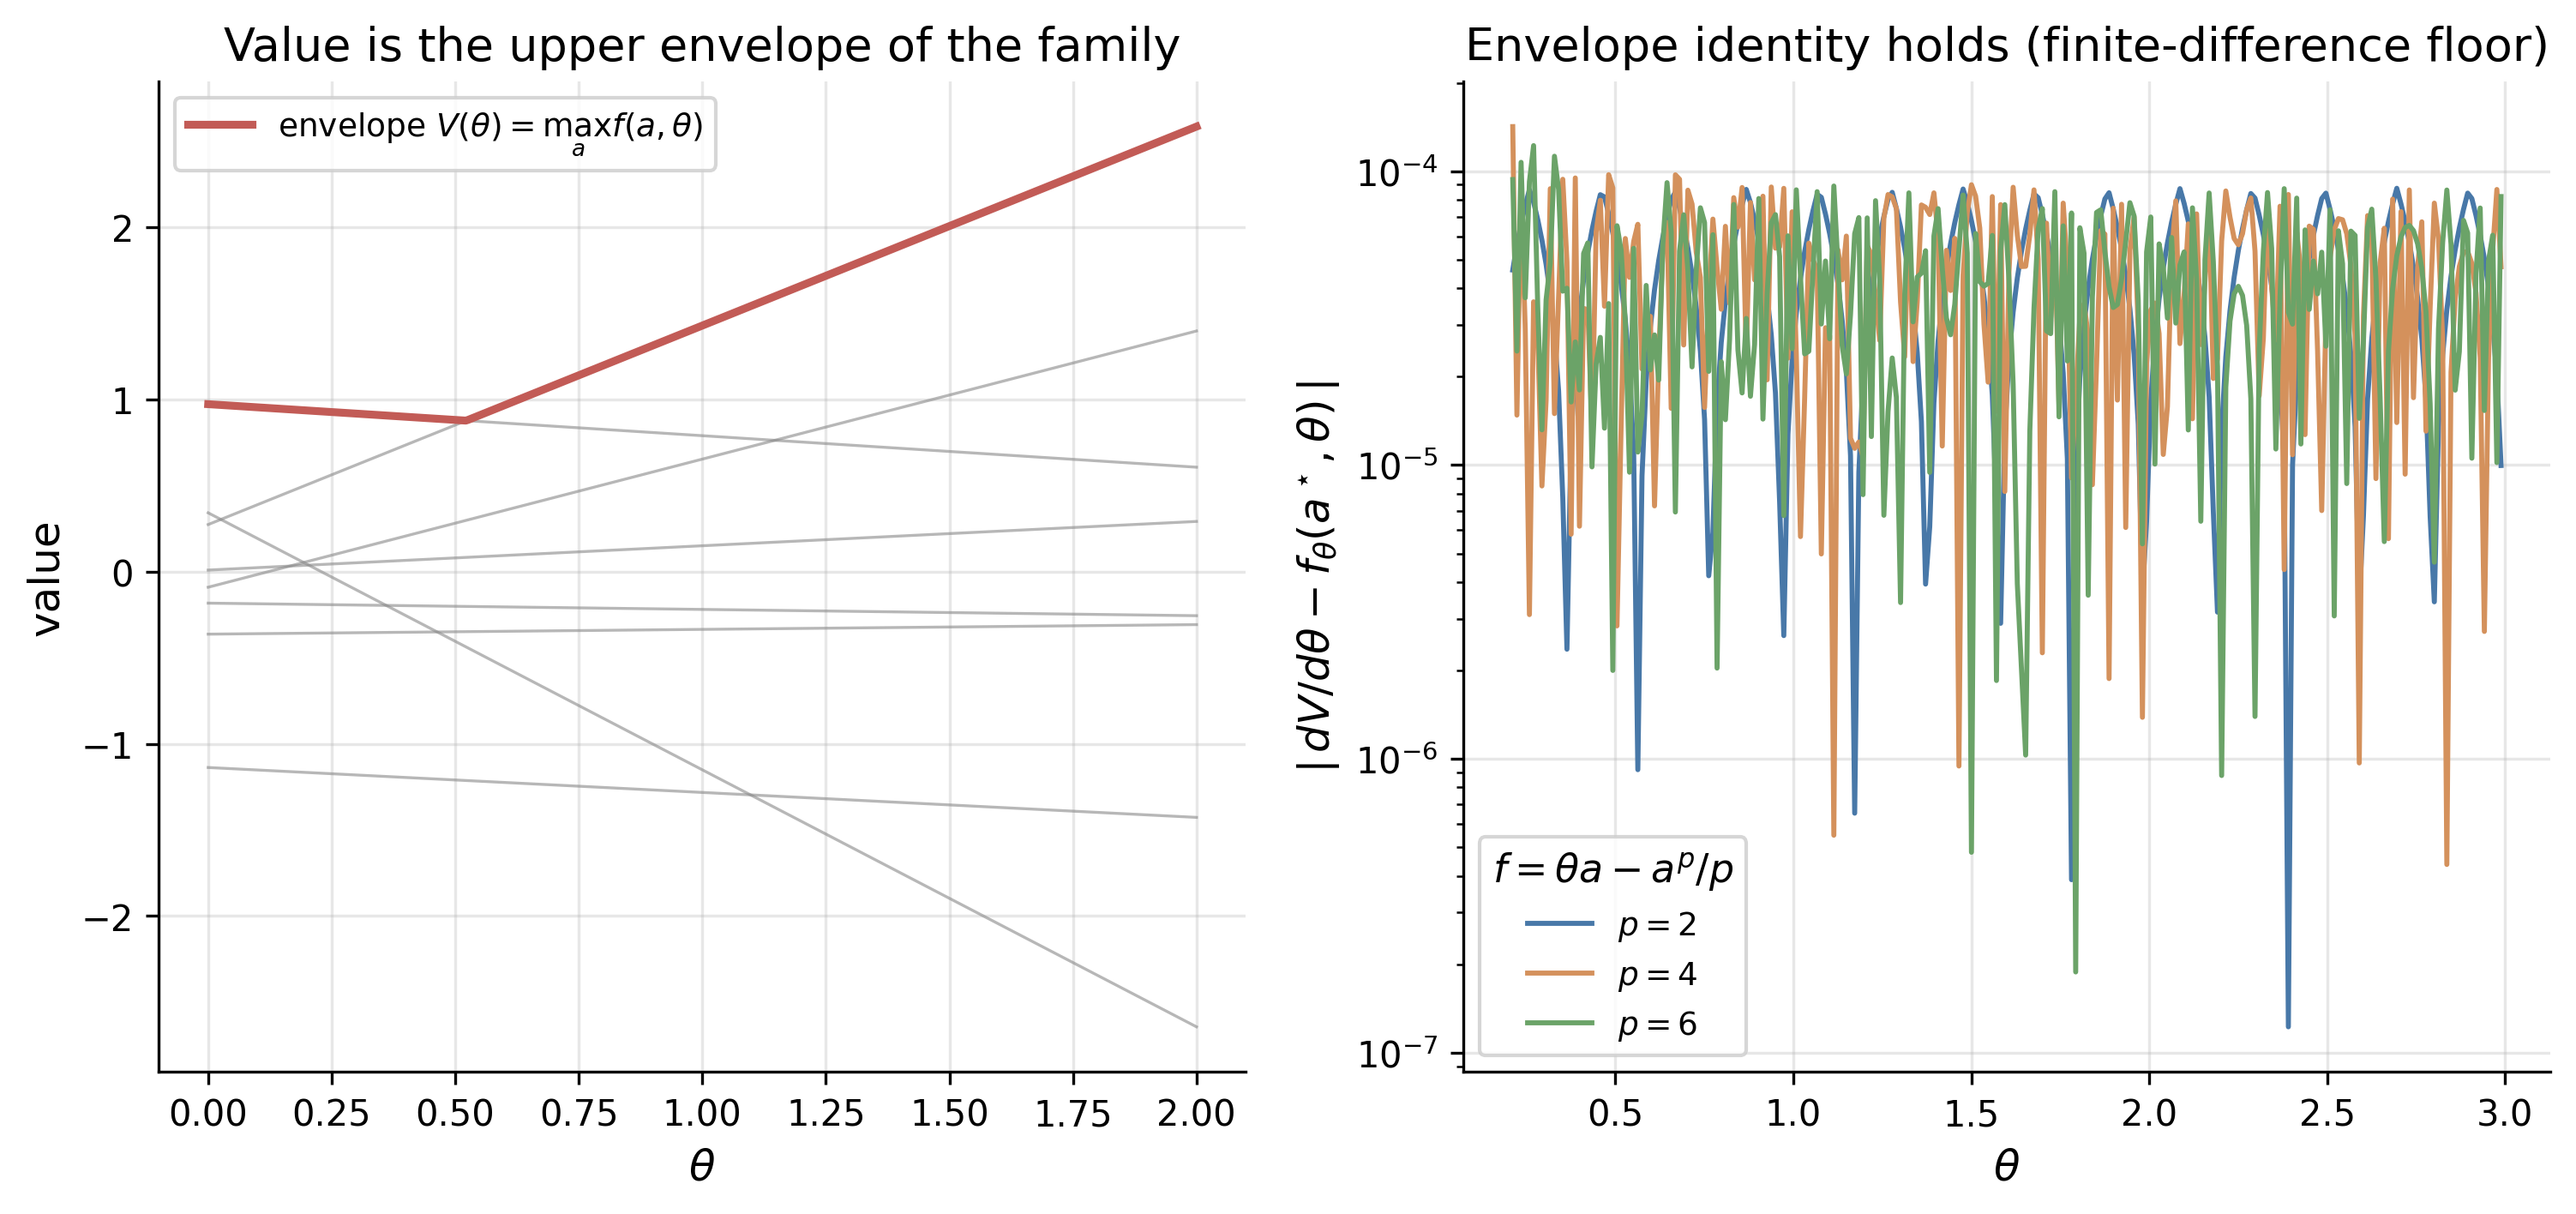
\includegraphics[width=0.95\textwidth]{../appA_preliminaries/sims/envelope_theorem.png}
\caption{Left: a family of linear payoffs $f(a, \theta) = \alpha_a + \beta_a \theta$ (thin) and their upper envelope $V(\theta) = \max_a f(a, \theta)$ (thick), which coincides with the active member on each segment and kinks where the maximizer switches. Right: the envelope residual $|dV/d\theta - \partial_\theta f(a^\star, \theta)|$ against $\theta$ for the smooth families $f = \theta a - a^p/p$, $p \in \{2, 4, 6\}$, on a log scale, at the finite-difference and grid-quantization floor.}
\label{fig:prelim_envelope}
\end{figure}

\begin{table}[h]
\centering
\caption{The envelope theorem $dV/d\theta = f_\theta(a^\star(\theta),\theta)$ checked on smooth conjugate families $f(a,\theta)=\theta a - a^p/p$, for which $a^\star(\theta)=\theta^{1/(p-1)}$. A central-difference derivative of the numerically maximized $V$, which uses no knowledge of $a^\star$, reproduces the partial $f_\theta(a^\star,\theta)=a^\star$ to the finite-difference floor; the numerical $V$ and $a^\star$ match their closed forms. The last row reports the line-family envelope, where the identity holds at every $\theta$ off the measure-zero kinks.}
\label{tab:prelim_envelope}
\begin{tabular}{lccc}
\hline
Family & Max envelope residual & Max $|V-V_{\mathrm{exact}}|$ & Max $|a^\star - a^\star_{\mathrm{exact}}|$ \\
\hline
$p=2$ & 8.75e-05 & 3.83e-09 & 8.75e-05 \\
$p=4$ & 1.42e-04 & 2.37e-08 & 8.74e-05 \\
$p=6$ & 1.22e-04 & 4.23e-08 & 8.65e-05 \\
\hline
Lines (off kinks) & identity holds on 1.000 of $\theta$ & \multicolumn{2}{c}{1.0 kinks per envelope} \\
\hline
\end{tabular}
\end{table}


\subsubsection{Lipschitz Continuity}

\begin{theorem}[Lipschitz continuity, \citet{nesterov2018}]
\label{thm:prelim_lipschitz}
A map $f$ between normed spaces is \emph{$L$-Lipschitz} if $\|f(x) - f(y)\| \leq L\|x - y\|$ for all $x, y$.\footnote{Lipschitz continuity is a uniform bound on how fast $f$ can change. A \emph{$\gamma$-contraction} is the special case $L = \gamma < 1$, the hypothesis of the Banach theorem in Section~\ref{prelim:fixedpoints}.} For a differentiable real-valued $f$ on $\mathbb{R}^n$ the least such constant is the supremum of the gradient norm,
\begin{equation}
L = \sup_x \|\nabla f(x)\|.
\label{eq:prelim_lipschitz}
\end{equation}
For a linear map $A$ the least constant is the induced operator norm $\|A\|$. In particular the policy-evaluation operator $T V = r + \gamma P V$ is $\gamma$-Lipschitz in the supremum norm, and the resolvent solve $r \mapsto (I - \gamma P)^{-1} r$ is $\tfrac{1}{1-\gamma}$-Lipschitz.
\end{theorem}

\begin{proof}
The plan is to read the Lipschitz constant of a smooth function off its gradient with the mean value theorem, and the constant of a linear map off its induced norm, then apply the second to the Bellman operator and its inverse. For a differentiable $f$ the mean value theorem gives, for some $\xi$ on the segment between $x$ and $y$,
\begin{align*}
|f(x) - f(y)| = |\nabla f(\xi)^\top (x - y)|
  &\leq \sup_z \|\nabla f(z)\|\, \|x - y\| && \text{(mean value theorem, Cauchy-Schwarz),}
\end{align*}
so $L \leq \sup_z \|\nabla f(z)\|$; letting $y \to x$ along the gradient direction makes the quotient approach $\|\nabla f(x)\|$, so the bound is tight and~\eqref{eq:prelim_lipschitz} holds. For a linear map $A$, $\|A(x - y)\| \leq \|A\|\,\|x - y\|$ by the definition of the induced norm, with equality approached along a maximizing direction, so the Lipschitz constant is $\|A\|$. Applying this to the Bellman operator, $T V - T V' = \gamma P (V - V')$, and since $P$ is row-stochastic, $\|P\|_\infty = 1$,
\begin{align*}
\|T V - T V'\|_\infty = \|\gamma P (V - V')\|_\infty
  &\leq \gamma \|P\|_\infty \|V - V'\|_\infty = \gamma \|V - V'\|_\infty && \text{(row-stochastic $P$).}
\end{align*}
For the resolvent, $(I - \gamma P)^{-1} = \sum_m (\gamma P)^m \geq 0$ entrywise and $(I - \gamma P)^{-1}\mathbf{1} = \tfrac{1}{1-\gamma}\mathbf{1}$, so every row sums to $\tfrac{1}{1-\gamma}$ and the supremum-norm operator norm is exactly $\tfrac{1}{1-\gamma}$.
\end{proof}

Lipschitz continuity is the condition every contraction argument in the survey rests on.\footnote{The $\gamma$-Lipschitz property of the Bellman operator is the contraction behind value iteration and temporal-difference learning (Section~\ref{sec:planning_learning}), and the $\tfrac{1}{1-\gamma}$ Lipschitz constant of the resolvent is the error-amplification factor in the approximate dynamic programming and robust value bounds of Section~\ref{sec:planning_learning} and Section~\ref{section:dist_robust_constrained}.} A learning update inherits a convergence rate only if the operator it applies does not stretch distances, which is exactly a Lipschitz bound with a constant below one. The Bellman operator supplies this with constant $\gamma$, the same $\gamma$ that reappears as the $\tfrac{1}{1-\gamma}$ amplification of any error fed into the value solve, which is precisely the Neumann-series bound of Theorem~\ref{thm:prelim_neumann}. Figure~\ref{fig:prelim_lipschitz} recovers the Lipschitz constant of several functions as the largest difference quotient and shows the Bellman error amplification tracking $\tfrac{1}{1-\gamma}$, and Table~\ref{tab:prelim_lipschitz} reports both to machine precision.

\begin{figure}[t]
\centering
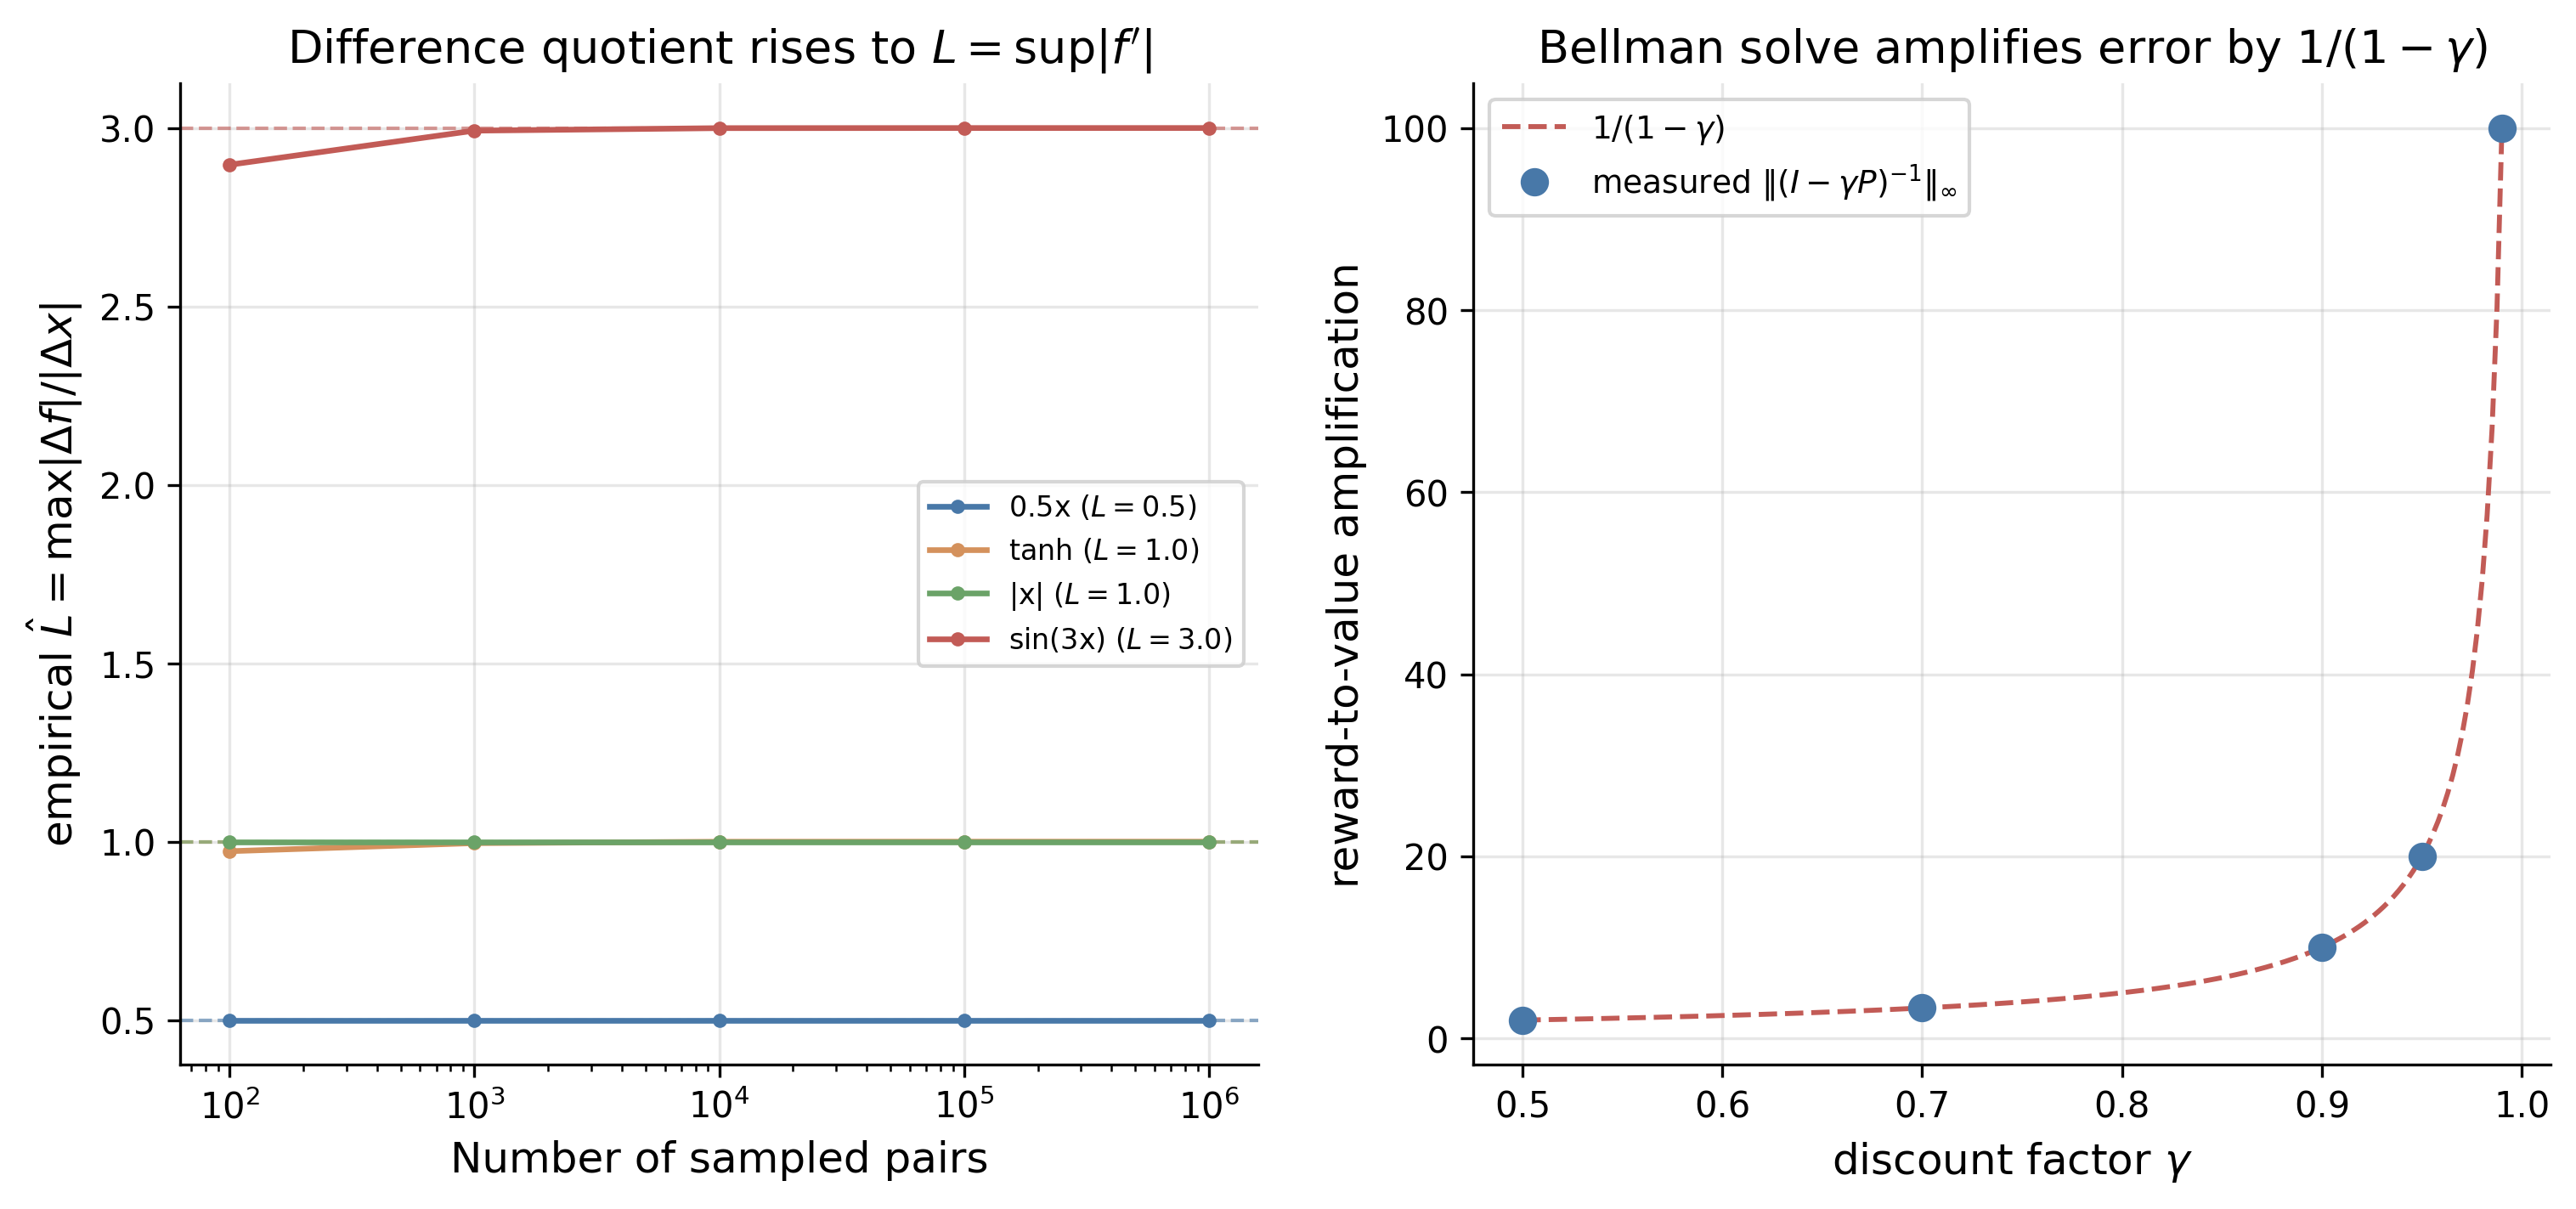
\includegraphics[width=0.95\textwidth]{../appA_preliminaries/sims/lipschitz_continuity.png}
\caption{Left: the empirical Lipschitz constant $\hat L$, the largest difference quotient $|f(x)-f(y)|/|x-y|$ over sampled pairs, rising to the analytic $L = \sup|f'|$ (dashed) from below for four scalar functions, on a log-scaled pair count. Right: the reward-to-value amplification $\|(I - \gamma P)^{-1}\|_\infty$ of the policy-evaluation solve against the discount factor $\gamma$ (markers), matching $1/(1-\gamma)$ (dashed).}
\label{fig:prelim_lipschitz}
\end{figure}

\begin{table}[h]
\centering
\caption{Lipschitz continuity, two checks. Top: the empirical Lipschitz constant $\hat L$ (largest difference quotient over sampled pairs) of four scalar functions rises to the analytic $L = \sup|f'|$ from below and never exceeds it. Bottom: the policy-evaluation Bellman operator $TV = r + \gamma P V$ is exactly $\gamma$-Lipschitz in the sup norm, and its fixed-point solve amplifies a reward perturbation by $\|(I-\gamma P)^{-1}\|_\infty = 1/(1-\gamma)$. Means over 12 sampling seeds and 20 random MDPs.}
\label{tab:prelim_lipschitz}
\begin{tabular}{lccc}
\hline
Function & Analytic $L$ & Measured $\hat L$ & $\hat L / L$ \\
\hline
$0.5x$ & 0.50 & 0.5000 & 1.0000 \\
$\tanh x$ & 1.00 & 1.0000 & 1.0000 \\
$|x|$ & 1.00 & 1.0000 & 1.0000 \\
$\sin(3x)$ & 3.00 & 3.0000 & 1.0000 \\
\hline
$\gamma$ & Operator Lip.\ ($=\gamma$) & Amplification & Theory $1/(1-\gamma)$ \\
\hline
0.5 & 0.5000 & 2.0000 & 2.0000 \\
0.7 & 0.7000 & 3.3333 & 3.3333 \\
0.9 & 0.9000 & 10.0000 & 10.0000 \\
0.95 & 0.9500 & 20.0000 & 20.0000 \\
0.99 & 0.9900 & 100.0000 & 100.0000 \\
\hline
\end{tabular}
\end{table}


\subsection{Fixed Points and Stochastic Approximation}
\label{prelim:fixedpoints}

Dynamic programming, temporal-difference learning, and their function-approximation variants all reduce to iterating an operator until it stops moving. Two results make that iteration converge. The Banach theorem handles the exact, deterministic operator. The Robbins-Monro theory handles its sampled, stochastic counterpart.

\subsubsection{The Banach Fixed-Point Theorem}

\begin{theorem}[Banach fixed-point theorem, \citet{banach1922}]
\label{thm:prelim_banach}
Let $(X, d)$ be a complete metric space.\footnote{A \emph{metric space} is a set $X$ with a distance $d(x,y)$ between points. It is \emph{complete} if every sequence whose terms bunch up without limit, a Cauchy sequence, actually has a limit inside $X$.} Let $T : X \to X$ be a $\gamma$-contraction, meaning there is a constant $\gamma \in [0, 1)$ with $d(Tx, Ty) \leq \gamma\, d(x, y)$ for all $x, y \in X$.\footnote{A \emph{contraction} is a map that pulls every pair of points strictly closer together, by at least the factor $\gamma < 1$. The reader should picture the Bellman operator, which shrinks the gap between any two value functions by $\gamma$ each time it is applied.} Then $T$ has a unique fixed point $x^\star = Tx^\star$, and for any starting point $x_0$ the iterates $x_{k+1} = Tx_k$ satisfy
\begin{equation}
d(x_k, x^\star) \leq \gamma^k\, d(x_0, x^\star).
\label{eq:prelim_banach_rate}
\end{equation}
\end{theorem}

\begin{proof}
The plan is to show the iterates form a Cauchy sequence, so completeness hands us a limit, and then to read off that the limit is the unique fixed point and that the error shrinks by $\gamma$ each step. First bound the distance between two consecutive iterates.\footnote{An \emph{iterate} is one term $x_k$ of the sequence built by applying $T$ over and over, starting from $x_0$ and setting $x_{k+1} = Tx_k$.} Applying the contraction to $x_k$ and $x_{k-1}$,
\begin{align*}
d(x_{k+1}, x_k) = d(Tx_k, Tx_{k-1})
  &\leq \gamma\, d(x_k, x_{k-1}) && \text{($T$ is a $\gamma$-contraction)} \\
  &\leq \gamma^k\, d(x_1, x_0) && \text{(apply the same step $k$ times).}
\end{align*}
Now bound the distance between any two iterates $x_m$ and $x_k$ with $m > k$.
\begin{align*}
d(x_m, x_k)
  &\leq \sum_{j=k}^{m-1} d(x_{j+1}, x_j) && \text{(triangle inequality)} \\
  &\leq d(x_1, x_0) \sum_{j=k}^{\infty} \gamma^j && \text{(previous bound, extend the sum)} \\
  &= \frac{\gamma^k}{1-\gamma}\, d(x_1, x_0) && \text{(geometric series).}
\end{align*}
The right-hand side tends to $0$ as $k \to \infty$. The iterates therefore bunch up without limit, so the sequence is Cauchy. Completeness gives a limit $x^\star \in X$.\footnote{This is the only place completeness is used, and it cannot be dropped. On the incomplete space $X = (0,1]$ the map $Tx = x/2$ is a contraction, yet its iterates march toward $0$, which is not in $X$, so no fixed point exists.} A contraction is continuous, so it commutes with the limit,
\begin{align*}
Tx^\star = T\Bigl(\lim_k x_k\Bigr) = \lim_k Tx_k = \lim_k x_{k+1} = x^\star .
\end{align*}
Thus $x^\star$ is a fixed point, a point the map leaves unchanged. For uniqueness, suppose $x^\star$ and $y^\star$ are both fixed points. Then
\begin{align*}
d(x^\star, y^\star) = d(Tx^\star, Ty^\star) &\leq \gamma\, d(x^\star, y^\star) && \text{(contraction),}
\end{align*}
so $(1-\gamma)\, d(x^\star, y^\star) \leq 0$. Since $\gamma < 1$, this forces $d(x^\star, y^\star) = 0$, and the two points coincide. Finally the rate. Apply the contraction to $x_{k-1}$ and the fixed point,
\begin{align*}
d(x_k, x^\star) = d(Tx_{k-1}, Tx^\star)
  &\leq \gamma\, d(x_{k-1}, x^\star) && \text{(contraction)} \\
  &\leq \gamma^k\, d(x_0, x^\star) && \text{(apply the same step $k$ times),}
\end{align*}
which is~\eqref{eq:prelim_banach_rate}.
\end{proof}

The dynamic-programming operators of the survey are all contractions in the supremum norm.\footnote{This theorem is the engine behind the convergence guarantees throughout the survey. The Bellman existence argument of Section~\ref{section:history}, value iteration and policy evaluation in Section~\ref{sec:planning_learning}, the minimax-Q and Nash-Q backups of Section~\ref{section:rl_games}, the robust and distributionally robust Bellman operators of Section~\ref{section:dist_robust_constrained}, and the model-based value operators of Section~\ref{section:world_models} each apply it to a contraction in the appropriate metric.} The policy-evaluation operator $T^\pi V = r^\pi + \gamma P^\pi V$ satisfies $\|T^\pi V - T^\pi V'\|_\infty \leq \gamma \|V - V'\|_\infty$, because $P^\pi$ is row-stochastic and averaging cannot increase the largest coordinate. The Bellman optimality operator inherits the same modulus (Section~\ref{sec:planning_learning}). Theorem~\ref{thm:prelim_banach} then supplies a unique value function and the geometric convergence of value iteration. Figure~\ref{fig:prelim_banach} iterates $T^\pi$ on random Markov reward processes at several discount factors. The measured per-step contraction factor tracks $\gamma$, and the error stays below the $\gamma^k$ envelope. The iterations needed to reach a fixed tolerance grow like $1/(1-\gamma)$ (Table~\ref{tab:prelim_banach}).

\begin{figure}[t]
\centering
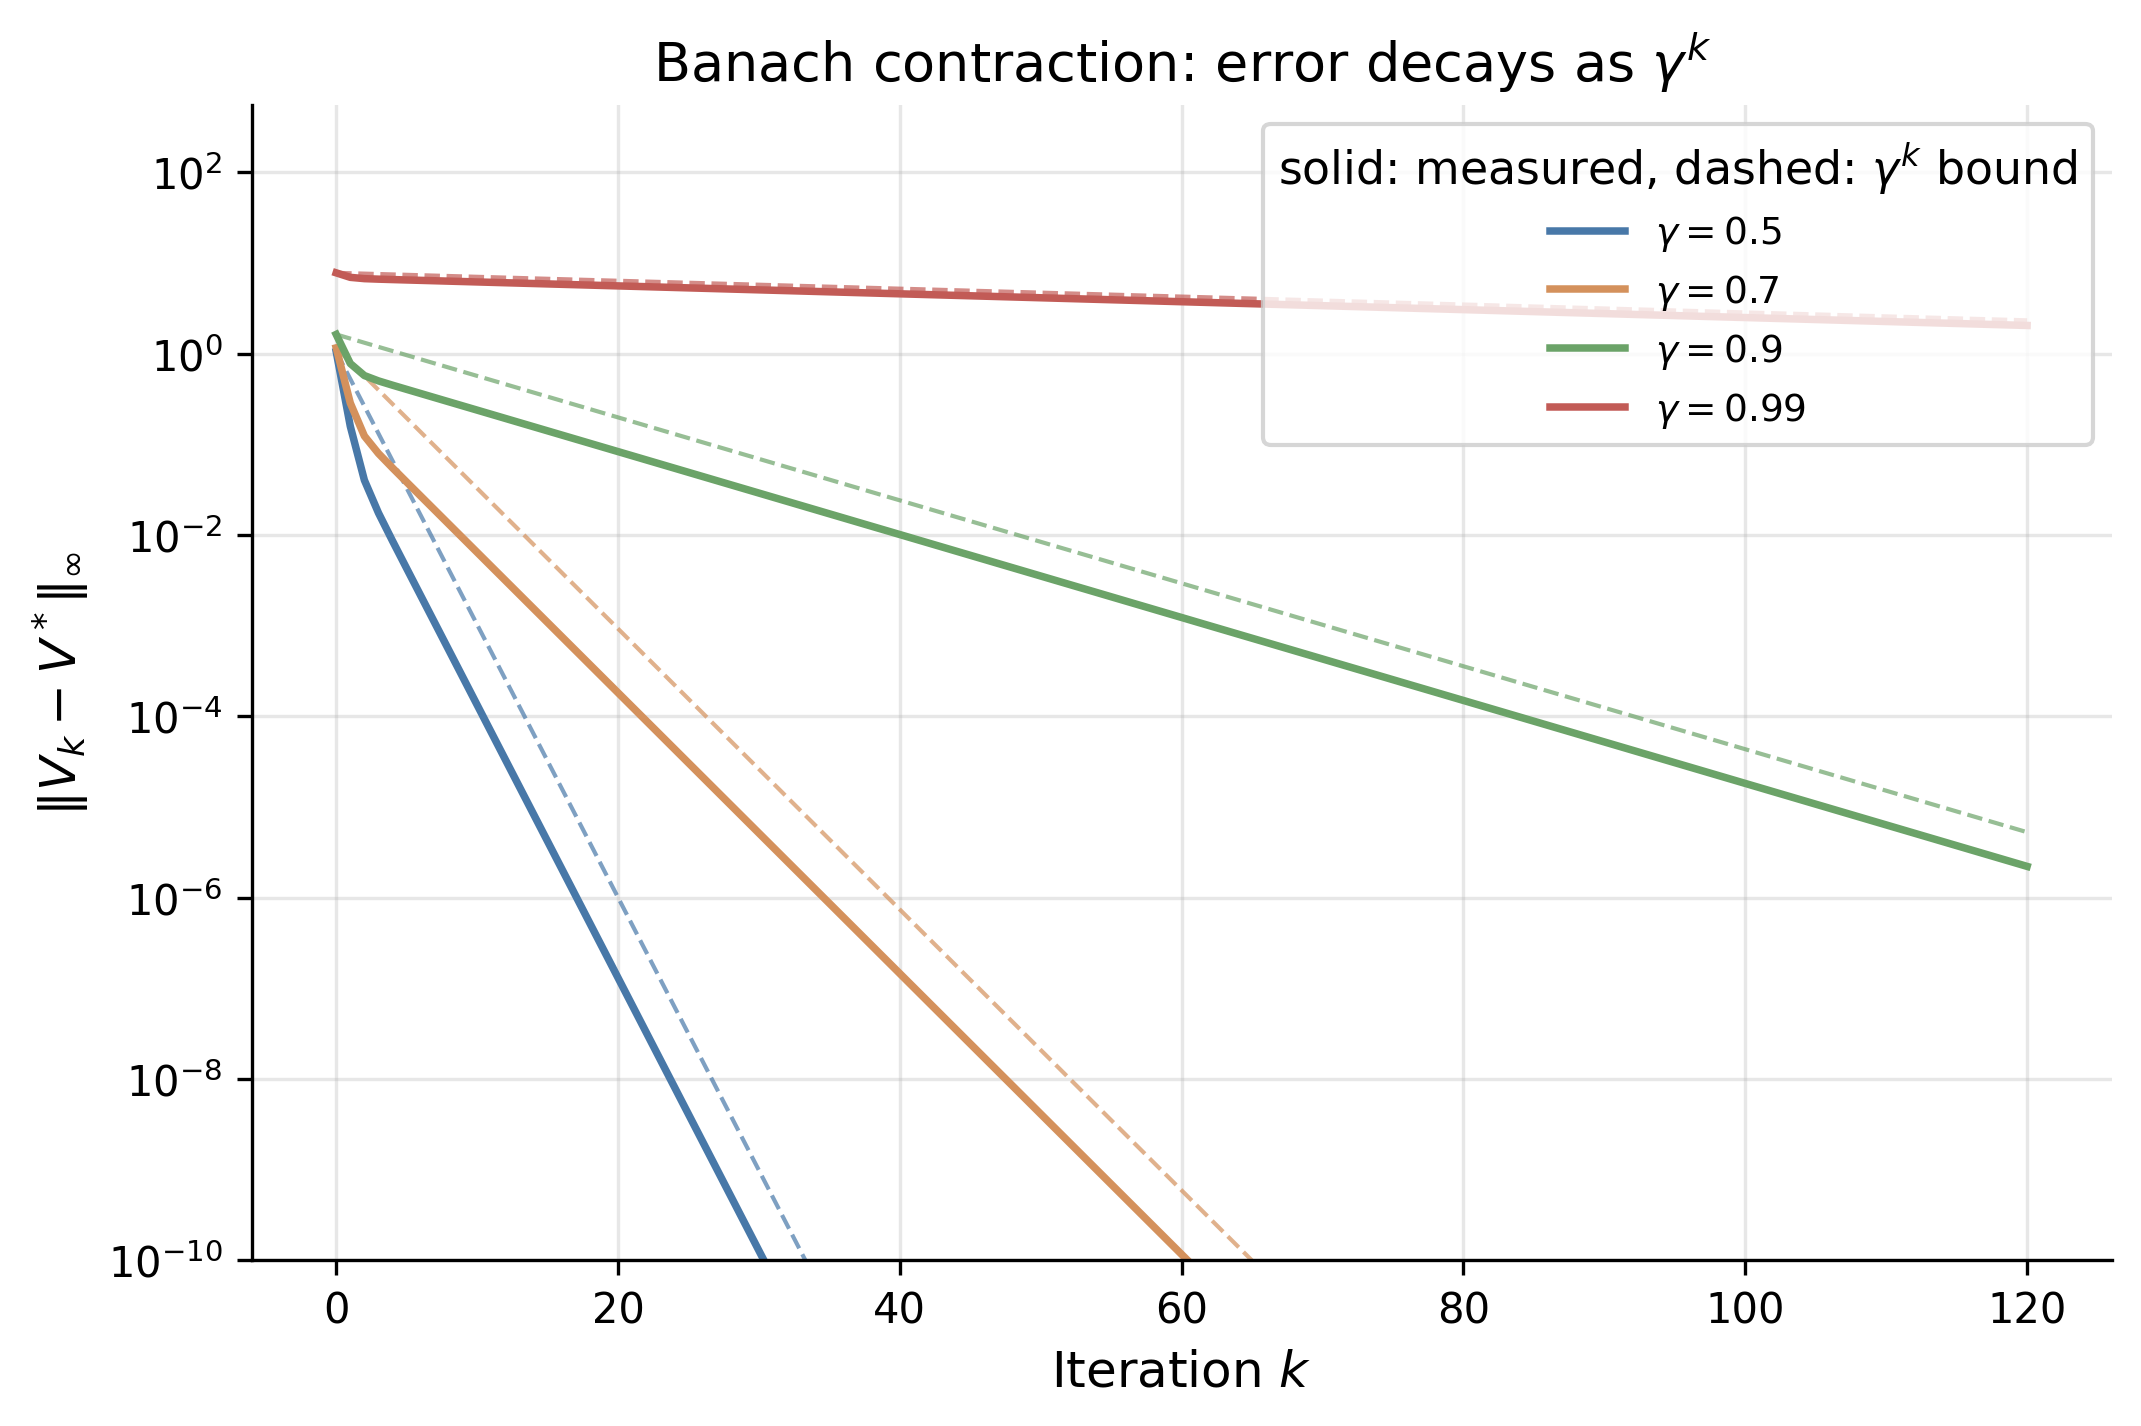
\includegraphics[width=0.78\textwidth]{../appA_preliminaries/sims/banach_contraction.png}
\caption{Supremum-norm error $\|V_k - V^\star\|_\infty$ of the iterates of the policy-evaluation operator $T^\pi V = r^\pi + \gamma P^\pi V$ on random 50-state Markov reward processes, averaged over 30 seeds, on a log scale. The solid curves show the measured error and the dashed curves the $\gamma^k \|V_0 - V^\star\|_\infty$ bound of Theorem~\ref{thm:prelim_banach}.}
\label{fig:prelim_banach}
\end{figure}

\begin{table}[h]
\centering
\caption{Banach fixed-point convergence of the policy-evaluation operator $TV = r + \gamma P V$ on a random 50-state Markov reward process. Measured contraction factor is the geometric mean of $\|V_{k+1}-V^*\|_\infty / \|V_k-V^*\|_\infty$. Iterations to $10^{-10}$ are reported both as measured (mean over the seeds that reach tolerance within 3000 iterations) and as predicted from $\log(\text{tol}/\text{err}_0)/\log\gamma$. Mean $\pm$ SE over 30 random MDPs.}
\label{tab:prelim_banach}
\begin{tabular}{ccccc}
\hline
$\gamma$ & Measured factor & Theory ($\gamma$) & Iterations to $10^{-10}$ (measured) & (predicted) \\
\hline
0.5 & 0.4626 $\pm$ 0.0026 & 0.50 & 30.4 & 33 \\
0.7 & 0.6776 $\pm$ 0.0018 & 0.70 & 60.1 & 65 \\
0.9 & 0.8951 $\pm$ 0.0005 & 0.90 & 212.6 & 223 \\
0.99 & 0.9899 $\pm$ 0.0000 & 0.99 & 2452.7 & 2495 \\
\hline
\end{tabular}
\end{table}


\subsubsection{Robbins-Monro Stochastic Approximation}

The Banach theorem governs the exact operator. Reinforcement learning almost never has the exact operator. It sees a single noisy sample of the Bellman target at each step. Stochastic approximation is what rescues convergence. It replaces the deterministic contraction with a noisy update whose conditional mean still contracts.

\begin{theorem}[Robbins-Monro convergence, \citet{Robbins1952}]
\label{thm:prelim_robbins_monro}
Let $g$ be a $\gamma$-contraction on $\mathbb{R}$ with fixed point $x^\star$. Let the iterates evolve as
\begin{equation}
x_{t+1} = x_t + \alpha_t\bigl(g(x_t) - x_t + w_t\bigr),
\label{eq:prelim_rm_update}
\end{equation}
where $w_t$ is a martingale-difference noise adapted to a filtration $\mathcal{F}_t$, with $\mathbb{E}[w_t \mid \mathcal{F}_t] = 0$ and conditional variance $\mathbb{E}[w_t^2 \mid \mathcal{F}_t] \leq \sigma^2$.\footnote{A \emph{filtration} $\mathcal{F}_t$ is the record of everything known by time $t$. A \emph{martingale-difference} noise is one whose average, given that record, is zero, so $w_t$ adds no systematic bias to the update.} If the step sizes satisfy the two Robbins-Monro conditions
\begin{equation}
\sum_{t} \alpha_t = \infty \qquad \text{and} \qquad \sum_{t} \alpha_t^2 < \infty,
\label{eq:prelim_rm_conditions}
\end{equation}
then $x_t \to x^\star$ almost surely.\footnote{\emph{Almost surely} means with probability one. The first condition keeps the steps large enough to travel any finite distance to the root. The second makes them shrink fast enough for the noise to average out.}
\end{theorem}

\begin{proof}
The plan is to show the squared error is an almost-supermartingale, so a convergence theorem for such processes pins it down, and the two step-size conditions then force the limit to be zero. Write $e_t = x_t - x^\star$ for the error and $d_t = g(x_t) - x_t$ for the drift. Because $g(x^\star) = x^\star$, the drift splits as $d_t = b_t - e_t$ with $b_t = g(x_t) - x^\star$, and the contraction bounds $|b_t| = |g(x_t) - g(x^\star)| \leq \gamma|e_t|$. Square the update~\eqref{eq:prelim_rm_update} and take the conditional expectation.
\begin{align*}
\mathbb{E}[e_{t+1}^2 \mid \mathcal{F}_t]
  &= e_t^2 + 2\alpha_t e_t\, \mathbb{E}[d_t + w_t \mid \mathcal{F}_t] + \alpha_t^2\, \mathbb{E}\bigl[(d_t + w_t)^2 \mid \mathcal{F}_t\bigr] && \text{(expand the square)} \\
  &= e_t^2 + 2\alpha_t e_t (b_t - e_t) + \alpha_t^2\, \mathbb{E}\bigl[(d_t + w_t)^2 \mid \mathcal{F}_t\bigr] && \text{($\mathbb{E}[w_t \mid \mathcal{F}_t] = 0$)} \\
  &\leq e_t^2 - 2\alpha_t(1-\gamma) e_t^2 + \alpha_t^2 K(1 + e_t^2) && \text{($e_t b_t \leq \gamma e_t^2$; second moment bounded).}
\end{align*}
The last line uses $e_t b_t \leq |e_t|\,|b_t| \leq \gamma e_t^2$ on the cross term and folds the bounded second moment of $d_t + w_t$ into a constant $K$.\footnote{The successor moment is $\mathbb{E}[(d_t + w_t)^2 \mid \mathcal{F}_t] = d_t^2 + \mathbb{E}[w_t^2 \mid \mathcal{F}_t] \leq d_t^2 + \sigma^2$. With $d_t = b_t - e_t$ and $|b_t| \leq \gamma|e_t|$ this is at most $(1+\gamma)^2 e_t^2 + \sigma^2$, so $K = \max\{(1+\gamma)^2, \sigma^2\}$ works.} Collecting the $e_t^2$ terms,
\begin{align*}
\mathbb{E}[e_{t+1}^2 \mid \mathcal{F}_t] \leq (1 + \alpha_t^2 K)\, e_t^2 - 2\alpha_t(1-\gamma) e_t^2 + \alpha_t^2 K .
\end{align*}
This is an almost-supermartingale.\footnote{An \emph{almost-supermartingale} is a nonnegative process that would decrease in conditional expectation, except for two small perturbations. Here both perturbations are $\alpha_t^2 K$, and both are summable because $\sum_t \alpha_t^2 < \infty$.} The Robbins-Siegmund theorem \citep{robbinssiegmund1971} applies and gives two conclusions.\footnote{The Robbins-Siegmund theorem is the almost-supermartingale convergence result behind Theorem~\ref{thm:prelim_martingale}. It is the probabilistic engine behind essentially every almost-sure stochastic-approximation proof.} First, $e_t^2$ converges almost surely to a finite limit. Second, $\sum_t \alpha_t(1-\gamma) e_t^2 < \infty$ almost surely. The second sum is finite while $\sum_t \alpha_t = \infty$, so the terms $e_t^2$ cannot stay bounded away from zero. Their $\liminf$ is zero. A convergent sequence whose $\liminf$ is zero has limit zero, so $e_t \to 0$ and $x_t \to x^\star$ almost surely.
\end{proof}

The reinforcement-learning algorithms of the survey are the multi-component version of~\eqref{eq:prelim_rm_update}.\footnote{This lemma, in the finite-index contraction form of \citet{jaakkola1994} (a Q-learning-adapted Dvoretzky theorem) and \citet{tsitsiklis1994}, is what the survey invokes to prove almost-sure convergence. It supports Q-learning and $\mathrm{TD}(\lambda)$ in Section~\ref{sec:planning_learning}, the Nash-Q backup of Section~\ref{section:rl_games}, the single-loop structural estimators of Section~\ref{section:rl_econ_models}, the constrained and robust dual iterations of Section~\ref{section:dist_robust_constrained}, the Dyna and model-based updates of Section~\ref{section:world_models}, and the adaptive-learning dynamics discussed in Section~\ref{section:conclusion}. The continuous-time ODE method and the two-timescale extension for actor-critic live in the same references.} The scalar contraction $g$ becomes a Bellman-type operator that contracts in the supremum norm. The update is applied only at the state-action pair visited on that step. The conditional-mean contraction may hold only approximately. The same argument still carries through. Figure~\ref{fig:prelim_robbins_monro} runs~\eqref{eq:prelim_rm_update} under four schedules. Only those satisfying both conditions in~\eqref{eq:prelim_rm_conditions} reach the root. A constant step size leaves a noise floor. An over-aggressive $1/t^2$ schedule stalls short, because the iterate can travel only a finite total distance (Table~\ref{tab:prelim_robbins_monro}).

\begin{figure}[t]
\centering
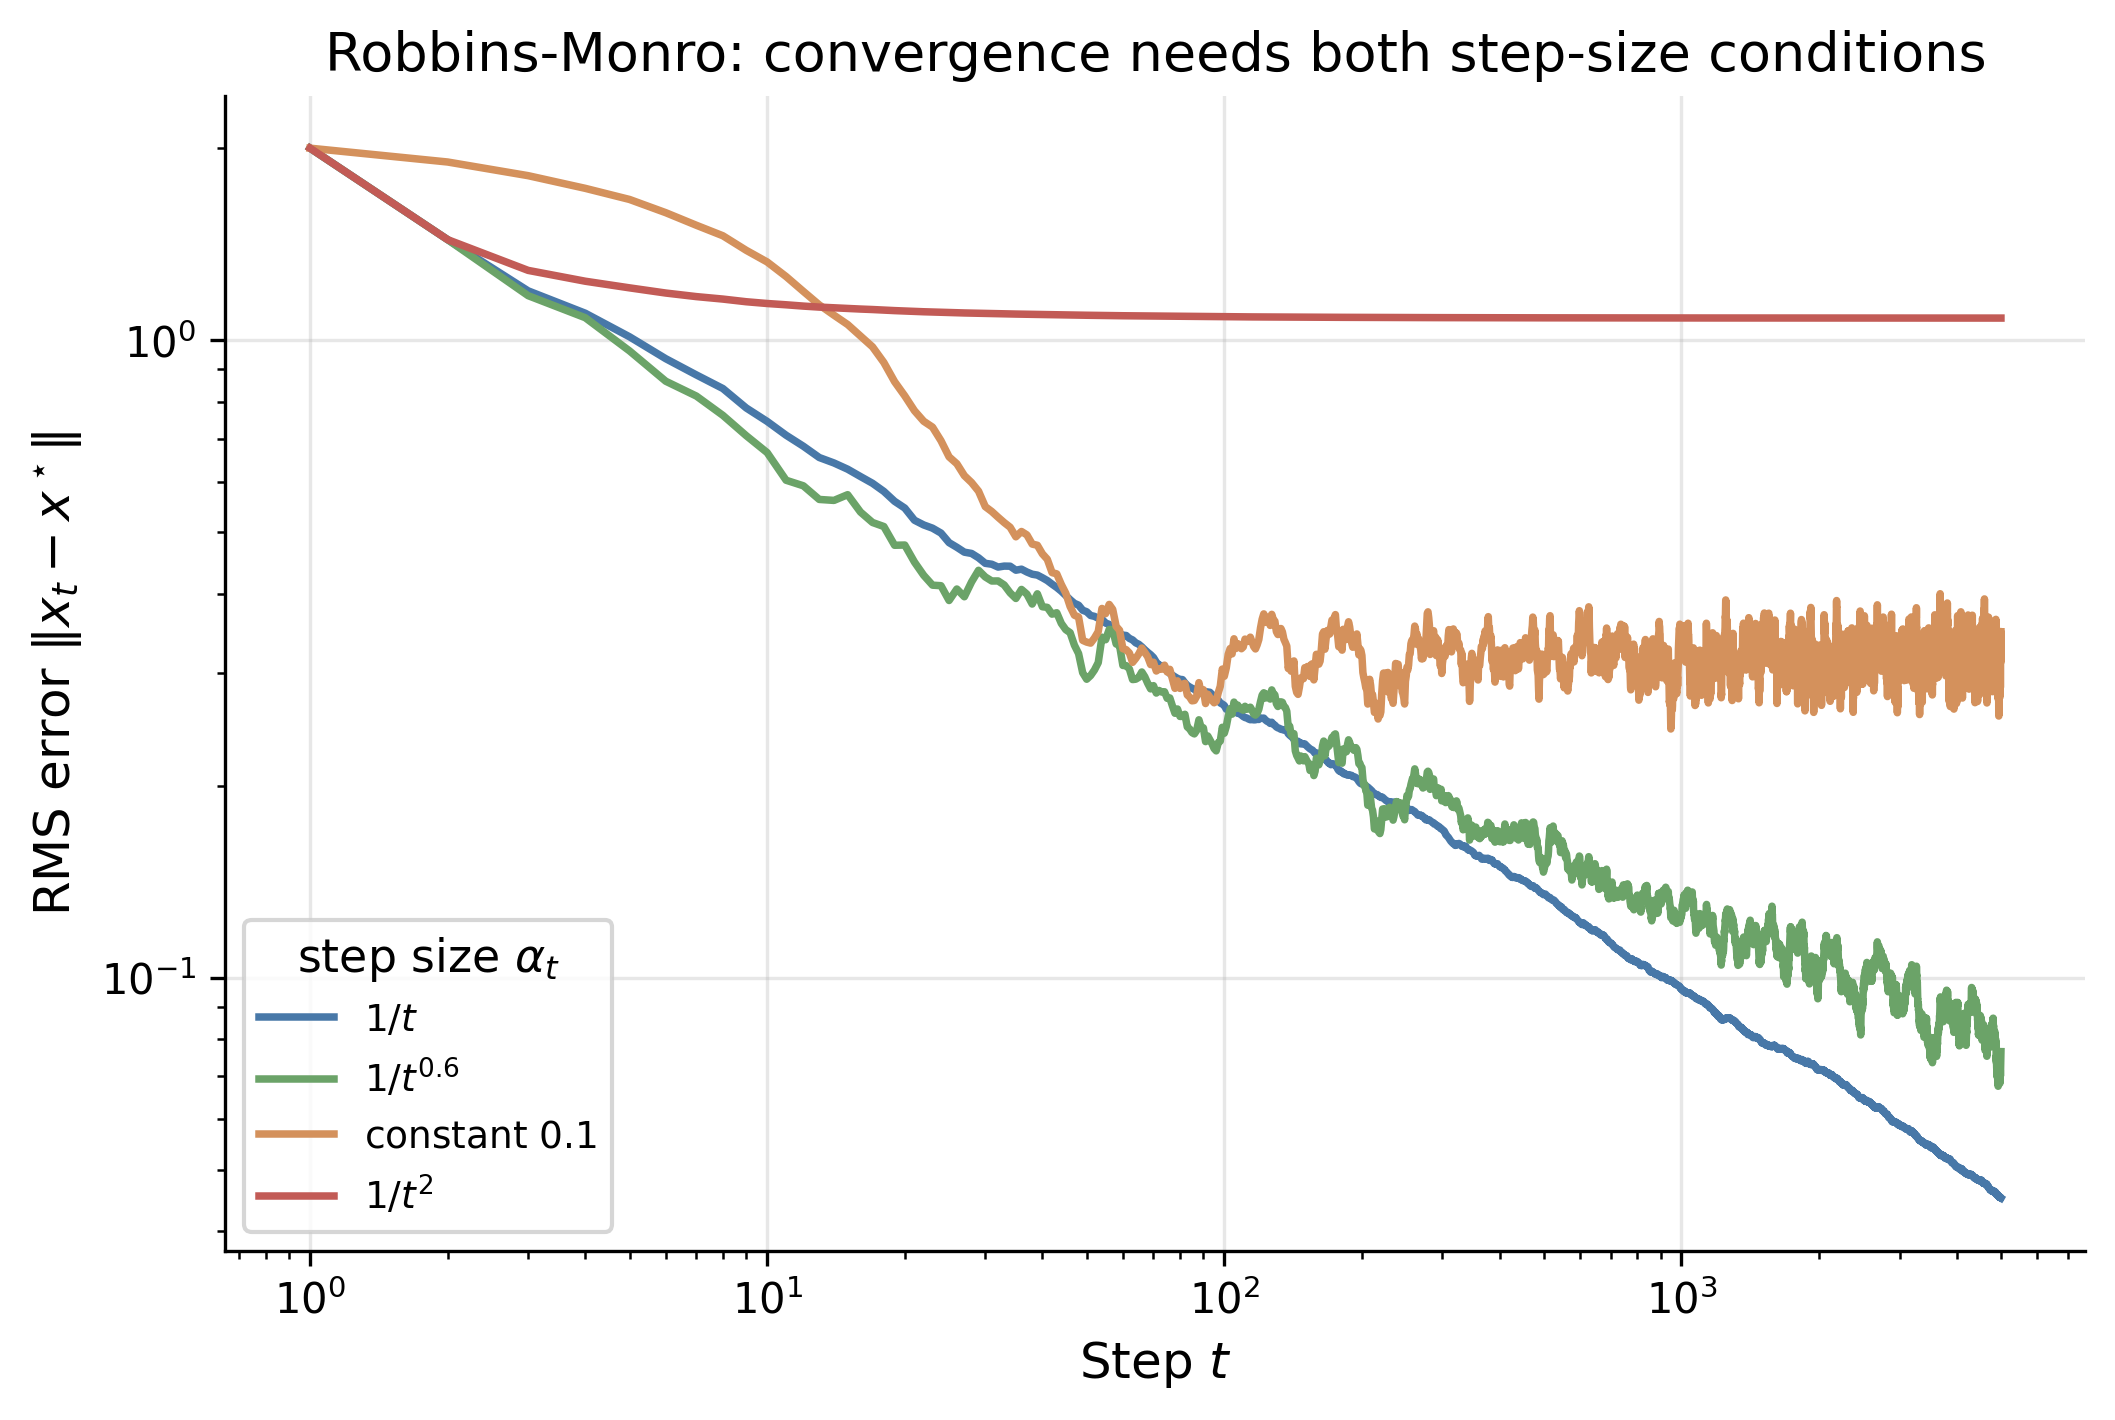
\includegraphics[width=0.78\textwidth]{../appA_preliminaries/sims/robbins_monro.png}
\caption{Root-mean-square error $\|x_t - x^\star\|$ of the stochastic-approximation recursion~\eqref{eq:prelim_rm_update} for the fixed point of $x = \gamma x + b$ under four step-size schedules, averaged over 100 seeds, on log-log axes. Only the two schedules that satisfy both Robbins-Monro conditions~\eqref{eq:prelim_rm_conditions} reach the root. The constant schedule settles into a noise floor. The $1/t^2$ schedule stalls.}
\label{fig:prelim_robbins_monro}
\end{figure}

\begin{table}[h]
\centering
\caption{Robbins-Monro stochastic approximation for the root of $x = \gamma x + b$ ($x^\star = 2$) with i.i.d. observation noise. A schedule converges to $x^\star$ only when $\sum_t \alpha_t = \infty$ and $\sum_t \alpha_t^2 < \infty$ both hold. Final RMS error over 100 seeds after 5000 steps.}
\label{tab:prelim_robbins_monro}
\begin{tabular}{lccc}
\hline
$\alpha_t$ & $\sum \alpha_t = \infty$ & $\sum \alpha_t^2 < \infty$ & Final RMS error \\
\hline
$1/t$ & yes & yes & 0.0451 \\
$1/t^{0.6}$ & yes & yes & 0.0766 \\
constant $0.1$ & yes & no & 0.3488 \\
$1/t^{2}$ & no & yes & 1.0827 \\
\hline
\end{tabular}
\end{table}
